% start the document

% specify the document layout and font size
%\documentclass[review,12pt]{elsarticle}
\documentclass[final,twocolumn,12pt]{elsarticle}
\usepackage[margin=1.5cm,includefoot]{geometry}
\usepackage{auto-paper}
\PassOptionsToPackage{refcheck}{auto-paper} %comment this out before submission
\usepackage{dcolumn}

\newcolumntype{d}[1]{D{.}{.}{#1}}

\zexternaldocument*{supp-frankenstein-2}
% Concatenate the different "values" .tex files
%RMSE values
% \newcommand{\baryrmse}{0.0242}
% \newcommand{\gprrmse}{0.0220}
% \newcommand{\idwrmse}{0.0345}
% \newcommand{\nnrmse}{0.0448}
% \newcommand{\avgrmse}{0.1302}
% %paper-data6
% \newcommand{\baryrmse}{0.0238}
% \newcommand{\gprrmse}{0.0218}
% \newcommand{\idwrmse}{0.0356}
% \newcommand{\nnrmse}{0.0445}
% \newcommand{\avgrmse}{0.1283}
%\newcommand{\gprrmsePercReduction}{83}
% paper-data9
\newcommand{\baryrmse}{0.0239}
\newcommand{\gprrmse}{0.0217}
\newcommand{\idwrmse}{0.0343}
\newcommand{\nnrmse}{0.0448}
\newcommand{\avgrmse}{0.1284}
\newcommand{\gprrmsePercReduction}{83.1}

%MAE values
% \newcommand{\barymae}{0.0145}
% \newcommand{\gprmae}{0.0145}
% \newcommand{\idwmae}{0.0223}
% \newcommand{\nnmae}{0.0307}
% \newcommand{\avgmae}{0.0965}
% %paper-data6
% \newcommand{\barymae}{0.0145}
% \newcommand{\gprmae}{0.0145}
% \newcommand{\idwmae}{0.0225}
% \newcommand{\nnmae}{0.0307}
% \newcommand{\avgmae}{0.0955}
%paper-data9
\newcommand{\barymae}{0.0145}
\newcommand{\gprmae}{0.0145}
\newcommand{\idwmae}{0.0223}
\newcommand{\nnmae}{0.0308}
\newcommand{\avgmae}{0.0959}

%\newcommand{\nnomega}{2.8709 \pm 0.69112}
\newcommand{\nnomega}{2.8702 \pm 0.69117}

\newcommand{\symtime}{76}

\newcommand{\nigprbrkrmse}{0.1471}

%Supplementary
\newcommand{\thr}{\SI{1.1}{\joule\per\square\meter}}
\newcommand{\sigthr}{\SI{1.1}{\joule\per\square\meter}}
\newcommand{\thrtwo}{\SI{1.2}{\joule\per\square\meter}}


%% main-frankenstein-2
\newcommand{\minsymdist}{$\sim$\SI{64.0}{\tobydeg}}
\newcommand{\percExplained}{$\sim$\SI{99.6}{\percent}}
\newcommand{\percFiveVsOne}{$\sim$\SI{70}{\percent}}
\newcommand{\dimOne}{$\sim$\SI{65}{\tobydeg}}

% figure info, etc. that can dynamically change (color of points, etc.)
\newcommand{\startpt}{red points}
\newcommand{\singlept}{magenta points}
\newcommand{\sympt}{dark blue points}
\newcommand{\singlesympt}{dark blue point}
\newcommand{\refpt}{white circle}
\newcommand{\vbordercolor}{black}
\newcommand{\vcellcolor}{light blue}
\newcommand{\inpt}{input}
\newcommand{\outpt}{prediction}
% \newcommand{\inptvar}{ninputpts}
% \newcommand{\distfn}{GBdist4}
\newcommand{\vfzorepo}{\gls{vfz} repository}
\newcommand{\mytitleone}{Five Degree-of-Freedom Property Interpolation of Arbitrary Grain Boundaries via \glsentrytitlecase{vfz}{long} Framework}
% \newcommand{\mytitletwo}{Properties of a \glsentrytitlecase{5dof}{long} \glsentrytitlecase{fz}{long} defined via \glsentrytitlecase{vfz}{long} Framework}
\newcommand{\mytitletwo}{$O_h$ \glsentrytitlecase{5dof}{long} \glsentrytitlecase{fz}{long} Properties via \glsentrytitlecase{vfz}{long} Framework}
\makeglossaries
\GlsXtrEnableEntryCounting{abbreviation}{3}
% \glssetcategoryattribute{abbreviation}{indexonlyfirst}{true}
\glssetcategoryattribute{abbreviation}{nohyper}{true}

% \setabbreviationstyle[abbreviation]{long-short}

% \glsenableentrycount
% \glssetcategoryattribute{abbreviation}{entrycount}{2}

\newabbreviation[longplural=five degrees of freedom]{5dof}{5DOF}{five degree-of-freedom}
\newabbreviation[longplural=three degrees of freedom]{3dof}{3DOF}{three degree-of-freedom}
\newabbreviation[longplural=degrees of freedom]{dof}{DOF}{degree of freedom}
\newabbreviation{ebsd}{EBSD}{electron backscatter diffraction}
\newabbreviation[longplural={grain boundaries}]{gb}{GB}{grain boundary}
\newabbreviation{fcc}{FCC}{face-centered cubic}
\newabbreviation{sem}{SEM}{scanning electron microscope}
\newabbreviation{fea}{FEA}{finite element analysis}
\newabbreviation{bcs}{BCs}{boundary conditions}
\newabbreviation[longplural={triple junctions}]{tj}{TJ}{triple junction}
\newabbreviation{gpr}{GPR}{Gaussian process regression}
\newabbreviation{gprm}{GPRM}{Gaussian process regression mixture}
\newabbreviation{ann}{ANN}{artificial neural network}
\newabbreviation{nn}{NN}{nearest neighbor}
\newabbreviation{rmse}{RMSE}{root mean square error}
\newabbreviation{mae}{MAE}{mean absolute error}
\newabbreviation{brk}{BRK}{Bulatov Reed Kumar}
\newabbreviation{gbed}{GBED}{grain boundary energy distribution}
\newabbreviation{gbcd}{GBCD}{grain boundary character distribution}
\newabbreviation{mfz}{MFZ}{misorientation fundamental zone}
\newabbreviation{bp}{BP}{boundary plane}
\newabbreviation{bpfz}{BPFZ}{boundary plane fundamental zone}
\newabbreviation{knn}{kNN}{k-nearest neighbor}
\newabbreviation{gbe}{GBE}{grain boundary energy}
\newabbreviation{gbo}{GBO}{grain boundary octonion}
\newabbreviation{nbo}{NBO}{no-boundary octonion}
\newabbreviation{oslerp}{oSLERP}{octonion Spherical Linear Interpolation}
\newabbreviation{loocv}{LOOCV}{leave-one-out cross validation}
\newabbreviation{kfcv}{kFCV}{k-fold cross validation}
\newabbreviation{seo}{SEO}{symmetrically equivalent octonion}
\newabbreviation{fex}{FEX}{file exchange}
\newabbreviation{idw}{IDW}{inverse-distance weighting}
\newabbreviation{fic}{FIC}{fully independent conditional}
\newabbreviation{svd}{SVD}{singular value decomposition}
\newabbreviation{gbc}{GBC}{grain boundary character}
\newabbreviation{fz}{FZ}{fundamental zone}
% \newabbreviation{pfz}{pFZ}{pseudo fundamental zone} % pfz replaced by vfz
% \newabbreviation{cmo}{CMO}{closed-mesh octonion} % cmo replaced by vfzo
\newabbreviation{vfz}{VFZ}{Voronoi fundamental zone}
\newabbreviation{vfzgbo}{VFZ-GBO}{Voronoi fundamental zone grain boundary octonion}
\newabbreviation{lobpcg}{LOBPCG}{locally optimal block preconditioned conjugate gradient}
\newabbreviation{lkr}{LKR}{Laplacian kernel regression}
\newabbreviation{ms}{MS}{molecular statics}
\newabbreviation{sst}{SST}{standard stereographic triangle}
\newabbreviation{ml}{ML}{machine learning}
\newabbreviation{doe}{DoE}{design of experiments}
\newabbreviation{ct}{CT}{coherent-twin}
% example abbreviations
% \newabbreviation{seo}{SEO}{symmetrically equivalent octonions}
%\newabbreviation[longplural={grain boundaries}]{gb}{GB}{grain boundary}

%example usage: \gls{gpr}
%example usage: \Gls{gpr} (capitalize first letter, only meaningful for first usage)
% \glspl{seo} --> symmetrically equivalent octonions OR SEOs
%^^^^^^^^^^^^^^^^^^^^^^^^^^^^^^^^^^^^^^^^^^^^^^^^^^^


\begin{document}
	
	\sloppy %to hopefully deal with whitespace better
	
	\begin{frontmatter}
		
		\title{\mytitletwo{}}
		
		\author[myu]{Sterling G. Baird\corref{cor1}}
\ead{ster.g.baird@gmail.com}
\author[myu]{Eric R. Homer}
\author[myu]{David T. Fullwood}
\author[myu]{Oliver K. Johnson}

\address[myu]{Department of Mechanical Engineering, Brigham Young University, Provo, UT 84602, USA}

\cortext[cor1]{Corresponding author.}

\date{October 2021}
		
		\begin{abstract}
		    We apply a newly developed \gls{vfz} framework to gain insights about \gls{gb} structure-property relationships in the \gls{5dof} space of cubic \glspl{gb}. We analyze the shape and size of a \gls{5dof} \gls{fz}, \gls{ms} energy uncertainty, property similarity of \glspl{gb} that are crystallographically "close" (i.e. correlations), and energy pathways through \gls{5dof} space. Considered together, these insights are important for managing trade-offs between accuracy, complexity, and design considerations for %experimental techniques such as
		    \gls{ebsd}/serial sectioning, \gls{hedm}, % and simulation methods such as
		    \gls{ms}, and \gls{dft}. In terms of the shape and size of a \gls{5dof} \gls{fz}, we discover that a \gls{fz} is smaller than expected at only $\sim$\SI{65}{\degree} in the largest principal component. Thus, a \SI{10}{\degree} difference between two \glspl{gb}, which may have previously been considered small, is actually quite large. %($\sim$\SI{15}{\percent} of the size of the \gls{fz}).
		    %Contrary to the classical definition of \glspl{gb} (a misorientation and plane normal),
		    We represent a \gls{gb} by five transformed Cartesian coordinates equipped with a Euclidean distance metric. Using this representation, we find that the \gls{fz} has a low aspect-ratio shape (i.e. width, length, height, etc. are similar) which is important for \gls{5dof} numerical differentiation. %We also show that \gls{ms} simulation uncertainty tends to be on the order of $\pm\sim$\SI{6}{\percent} when global optimization is omitted and that the max uncertainty is $\pm\sim$\SI{25}{\percent}.
		    Semivariogram and numerical optimization methods reveal that \gls{gbe} in Ni and Fe are globally correlated within $\sim$\SIrange{6}{8}{\degree} in the \gls{gbo} sense (multiply by 2 to convert to tilt angle). For local correlation lengths of high-symmetry \glspl{gb} of interest, we notice significant variation relative to global correlation lengths and an inverse relationship with the Brandon criteria. %A common assumption is that \num{10}$-$\SI{15}{\degree} spacing for experimental or simulated sample sets and simulation/characterization errors on the order of $\sim$\SI{10}{\percent} are reasonable.
		    % We demonstrate that commonly used spacing (\SIrange{10}{15}{\degree}) or error ($\sim$\SI{10}{\percent}) lead to inaccurate structure-property models and excessive smoothing. We suggest that %in order to draw more substantive conclusions about \gls{gb} behavior using crystallographic \gls{gb} structure-property models,
		    We suggest that property data with no more than $\pm\sim$\SI{3}{\percent} error and point sets with \glspl{gb} that are no more than $\sim$\num{3}$-$\SI{4}{\degree} apart should be used and then paired with high-fidelity interpolation strategies. Finally, in terms of dynamic material behavior, direct paths through \gls{5dof} space for Ni suggest that a certain low-energy $\Sigma7$ \gls{gb} may transform into the frequently observed $\Sigma3$ \gls{ct} \gls{gb}  %with monotonically decreasing energy (i.e. thermodynamically favorable), and this
		    which may be interesting to verify by experiment or simulation.
		\end{abstract}
		
% 		\begin{abstract}
% 			We apply a newly developed \gls{vfz} framework to gain insights about grain boundary structure-property relationships in the \gls{5dof} space of cubic \glspl{gb}. %the nature of a \gls{5dof} \gls{fz} for cubic $O_h$ \glspl{gb}. %The \gls{vfz} framework offers an advantage over other \gls{5dof} based property interpolation methods because it is defined via continuous, Euclidean coordinates and results in rapid distance calculations. %it is constructed as a point set in a manifold. This means that
% %			directly computed Euclidean distances approximate the original \gls{gbo} distance with significantly reduced runtime ($\sim$7 CPU minutes vs. 153 CPU days for a $\num{50000}\times\num{50000}$ pairwise-distance matrix). %this is where some fundamental insights probably need to be addressed before losing certain readers' attention
% 			%Aided by the increased computational efficiency of the \gls{vfz} framework,
% 			We determine the dimensions of a large $O_h$ \gls{vfz} point set, for which the maximum dimension is \dimOne{}. % after applying a \gls{svd} transformation. We also find that \gls{nn} distances for cubochorically sampled \glspl{gb} are normally distributed.
% 			\percExplained{} of the variance is explained by the first 5 \gls{svd} transformed coordinates % of the $O_h$ \glspl{vfzgbo},
% 			indicating that despite being originally defined by 8D Cartesian coordinates, 5D Cartesian coordinates and Euclidean distances may be sufficient to describe \glspl{gb} with respect to crystallographic "closeness". This is in contrast to the classical definition of \gls{5dof} coordinates via inharmonious combination of two very different mathematical objects: a rotation (misorientation) and a vector (plane normal). The 5th transformed dimension is \percFiveVsOne{} the size of the 1st dimension, giving a rough indication of the shape of a \gls{5dof} \gls{fz} (i.e. low aspect-ratio). % with a mean (\SI{}{\degree}) of approximately $2.5025\times10^{-5} x-1.27396 \log (x)+15.4499, x\in \{388,50000\}$ where $x$ is the number of \glspl{gb}.
% 			%This increased efficiency facilitates lower interpolation error through the use of significantly more input data.
% 			%We perform \gls{gbe} interpolation for a non-smooth validation function on sets of up to \num{50000} \glspl{gb} using four interpolation methods: barycentric interpolation, \gls{gpr} or Kriging, \gls{idw}, and \gls{nn} interpolation. % These are evaluated for \num{50000} random \inpt{} \glspl{gb} and \num{10000} random \outpt{} \glspl{gb}.
% 			%The best performance was achieved with \gls{gpr}. %, which results in a reduction of the \gls{rmse} by \calcnum{(\avgrmse-\gprrmse)/\avgrmse*100}\%. % relative to \gls{rmse} of a constant, average model.
% 			%We then use \gls{gpr} to interpolate simulated bi-crystal datasets for Fe and Ni and demonstrate better than and similar performance to prior work, respectively. % Interpolation on a large, noisy, \gls{ms} Fe simulation dataset improves performance by \SI{34.4}{\percent} compared to \SI{21.2}{\percent} in prior work, and we discover that
% 			We identify repeated \glspl{gb} in a large Fe simulation dataset which in turn enables us to estimate the intrinsic uncertainty in the context of experimental measurements and metastable \gls{gb} states. % (\SI{0.065}{\J\per\square\m}).
% 			%We find that the noise and non-uniform sampling make it difficult to resolve low \gls{gbe} (i.e. cusps) and to validate the model. %Interpolation on a small, low-noise \gls{ms} Ni simulation dataset is similar to interpolation results previously reported, and
% 			%For the small, low-noise Ni simulation data, we resolve cusps with high accuracy, but uncertainty may be high in regions far from the input data. The trade-offs between noise, dataset size, sampling scheme, and repeat measurements must be carefully managed.
% 			\Gls{gpr} allows us to estimate the correlation lengths of the Ni and Fe datasets to be $\sim$\SIlist{7.4;8.3}{\degree}, respectively, compared with a traditionally accepted value of $\sim$\SI{10}{\degree}. When the Ni dataset is assumed to have low-noise, the correlation length drops to $\sim$\SIlist{1.9}{\degree}. This indicates that traditional models which rely on the \SI{10}{\degree} assumption are too smooth. Relative to the size of a \gls{vfz}, these correlation lengths suggest that \glspl{gbe} are typically correlated within $\sim$\SI{11}{\percent} to \SI{18}{\percent} of the \gls{5dof} \gls{fz}, regardless of whether the sample is FCC or BCC. That is, grids with spacing close to or larger than this lead to less effective \gls{5dof} models. % (\SI{57.6}{\percent} vs. \SI{56.4}{\percent}).
% 			% BRANDON'S CRITERIA
% 			We analyze structure-property paths between the $\Sigma3$ \gls{ct} \gls{gb} and other low-Sigma \glspl{gb} of interest. The \gls{5dof} path between the FCC-Ni \gls{ct} $\Sigma3$ cusp and a $\Sigma7$ cusp are connected (i.e. a direct path exists without an energy barrier), suggesting that the $\Sigma7$ cusp will spontaneously transform into the global minimum \gls{ct} $\Sigma3$ cusp (i.e. the transformation is thermodynamically favorable with respect to energy minimization). Future work involves probing other cubic and non-cubic symmetries, alloys, and properties such as mobility. % which can be applied to future datasets for a variety of \gls{gb} properties. % which has potential for the creation of advanced \gls{gb} structure-property models for alloys and cubic/non-cubic crystallographic point groups. %The \gls{vfz} framework offers advantages for computing distances between \glspl{gb}, estimating property values for arbitrary \glspl{gb}, and modeling surrogates of computationally expensive \gls{5dof} functions and simulations.
% 		\end{abstract} %too detailed, too mathy, not enough roadmap
		
		% Some of the less-emphasized fundamental contributions to understanding (that maybe I should incorporate into the abstract/emphasize more) are:
		
		% - an estimate of the intrinsic error of an Fe simulation dataset (Section 3.1.1. Experimental and Simulation Error, see also Figure S11). The data is estimated to have an intrinsic error on the order of 0.065 J m^-2.
		
		% - 1NN distribution and kNN distances for 50000 random cubochorically sampled points in a VFZ (Figure 2). If you take 50000 random points, the average NN distance is 2.87 +/- 0.69 deg and the distribution is Gaussian. Typically, the first 10 NNs have average NN distances less than 5 deg.
		
		% - average 1NN distance as a function of set size (Figure 5). I.e. how closely spaced is the data based on a random set of points?
		
		% - the maximum dimension of an O_h VFZ is ~60 deg (2.1.3. Distance Calculations in the Voronoi Fundamental Zone, see also Figure S1), i.e. the largest minimum distance path for O_h point group symmetry is ~60 deg. Puts correlation lengths into perspective (10 deg is pretty large).
		
		% - large amounts of noise in the input data make it difficult to resolve deep cusps accurately (sort of a negative to large, noisy datasets --> smaller, low-noise datasets are generally to be preferred)
		
		% - a \gls{gb} correlation length of 10 degrees is probably an overestimate. The GPR model gives a correlation length of 7.4 degrees for the Olmsted Ni GBE data. If you assume near-zero input noise, the correlation length drops to ~2 degrees. If you take 50,000 points from the BRK model, the fitted correlation length is 10.5 degrees.
		
		% - I could swap out "A" and "B" with Sigma 3 and Sigma 7 to show that they're connected, or with Sigma 3 and Sigma 5 to show two cusps. Also, minimum energy path vs. minimum distance path vs. VFZ path. An application for earth mover's distance?
		
		% we have an estimate for the most likely function value (1.16 J/m^2) in a random cubochoric sense for the BRK function.
		
		% the first \gls{5dof} FZ with continuous coordinates
		
		\begin{keyword}
			grain boundary energy \sep five degree-of-freedom \sep structure-property model \sep machine learning \sep octonion % \sep Metastability \sep Grain Boundary Distance \sep Grain Boundary Energy
		\end{keyword}
		
	\end{frontmatter}
	
	%\linenumbers %to help reviewers
	
	\section{Introduction} \label{sec:intro}
	
	When subjected to plastic deformation and/or elevated temperatures, the crystallographic character of grain boundaries (GBs) in polycrystalline microstructures can change to reduce the total system energy \cite{bachurinGrainRotationDislocation2012,barrales-moraImpactGrainBoundary2014,harrisGRAINROTATIONTHIN,klingerShapeEvolutionSurface2011,upmanyuSimultaneousGrainBoundary2006a}. These energy minimizing transformations of \gls{gb} crystallography constitute trajectories or paths along the \gls{gb} energy landscape, which is a function over the 5-dimensional (5D) \gls{gb} character space. Consequently, to understand, model, and predict such transformations and their effects on microstructure evolution, it is necessary to understand these paths and the relationships between \glspl{gb} that are near each other in that space.
	
	Examples of such spontaneous energy minimizing changes to \gls{gb} character include the rotation of the \gls{gb} plane to achieve equilibrium at triple junctions \cite{Herring:1951tm,rowenhorstMeasurementsGrainBoundary2005a}---both those formed by the intersection of three \glspl{gb} within a polycrystal and those formed between a \gls{gb} and two free surfaces at the exterior of a microstructure. It is this phenomenon that is exploited to produce the quarter- and half-loop bicrystal geometries used in classic constant-driving-force \gls{gb} migration experiments \cite{brandenburgEffectInclinationDependence2013,furtkampGrainBoundaryMigration1998,gottsteinGrainBoundaryMigration,ivanovImpactBoundaryOrientation2004,molodovEffectPressureMigration1984,molodovMOBHJTYTILTGRAIN}. The inclination of the \gls{gb} plane can also change during \gls{gb} migration [REF], faceting into different combinations of \gls{gb} planes to reduce energy \cite{ramasubramaniamEvolutionFacetedGrainboundary2005}, or upon the disappearance of a grain during grain growth (which requires establishment of new equilibrium configurations at the newly formed triple junctions). This class of energy minimizing changes to \gls{gb} character constitute paths through the \gls{gb} energy landscape that are restricted to two-dimensional sub-manifolds (the \gls{gb} plane fundamental zone (FZ) for a fixed misorientation).
	
	Another class of energy minimizing changes to \gls{gb} character are illustrated by the phenomenon of grain rotation \cite{basakTwodimensionalStudyCoupled2014,bernsteinInfluenceGeometryGrain2008,fujitaDirectObservationSubgrainGrowth1961,huangGrainRotationLattice2015,sharmaObservationChangingCrystal2012,trauttCapillarydrivenGrainBoundary2014,ueharaAtomisticStudyGrain2008,upmanyuSimultaneousGrainBoundary2006,upmanyuSimultaneousGrainBoundary2006b,weissmannMechanismRecrystallizationAluminum1958}, which can occur during high-temperature plastic deformation \cite{ashbyApplicationBoundTheorems1978,gifkinsGrainboundarySlidingIts1976,herringDiffusionalViscosityPolycrystalline1950,leeStrainRateDependent1970,matsukiRelativeMotionGrains1977,nabarroSteadystateDiffusionalCreep1967,zelinGeometricalAspectsSuperplastic1996} or recrystallization \cite{liPossibilitySubgrainRotation1962}, as well as at lower temperatures in nanocrystalline materials \cite{wangGrainRotationMediated2014}. The primary feature of grain rotation is the change in crystal orientation of one grain relative to its neighbors resulting in lower-energy \glspl{gb} between them. However, when the misorientation between two grains changes there will also be an accompanying change to the \gls{gb} plane inclination\footnote{Even if the \gls{gb} plane remains fixed in the macroscopic reference frame, a change in the \gls{gb} misorientation results in a change of the \gls{gb} normal in the crystal reference frame, which is the physically relevant reference frame.}. Consequently, such \gls{gb} character transformations represent more general paths through the 5D \gls{gb} character space that are not restricted to any misorientation or boundary plane subspaces.
	
	Until recently, models for \gls{gb} energy that depend on their full 5D crystallographic character were unavailable. Bulatov, Reed, and Kumar (BRK) \cite{bulatovGrainBoundaryEnergy2014} developed a fully 5D \gls{gb} energy model by fitting a closed-form function to \gls{gb} energies from a database \cite{olmstedSurveyComputedGrain2009a} of 388 \glspl{gb} in several materials. This function has been employed in a variety of applications to study mesoscale microstructure phenomena like X [REF], Y [REF], and Z [REF]. We recently developed a general approach, called the Voronoi fundamental zone (VFZ) framework, for inferring \gls{gb} structure-property models from \gls{gb} structure-property databases \cite{bairdFiveDegreeoffreedomProperty2021}. 
	
	In this work we present 5D \gls{gb} structure-property models for FCC Ni and BCC Fe developed using the VFZ framework. We also study correlations in \gls{gb} energy as a function of crystallographic distance. We use the VFZ framework to give context to \gls{gb} property correlation lengths\footnote{Correlation length in the context of \glspl{gb} has been described as the degree to which boundaries with the same
    macroscopic geometrical degrees of freedom in different materials have related properties \cite{olmstedSurveyComputedGrain2009}. } and find that previous estimates are likely too high for low-noise, computational \gls{gbe} calculations. Finally, we investigate general paths through the \gls{gb} energy landscape and show qualitatively distinct types of relationships between important types of GBs.
	
% 	Maybe consider choosing terminal \glspl{gb} for the paths to investigate this-> research shows that grain rotation only occurs for misorientations that are pure-tilt in character (ones with general tilt-twist character do not show grain rotation). We could test or show why this is the case (my guess is there would be grain rotation for some general GBs-> those for which there is a strictly downhill path). Maybe look at a sigma 5, which is a minimum in the symmetric tilt space so it likely would not rotate, but maybe it has another downhil path that leaves the symmetric tilt space? Or maybe we could find a general \gls{gb} that we think would show grain rotation because it has a downhill path.
	
% 	papers that discuss changes to \gls{gb} character to minimize energy
% 	https://www.sciencedirect.com/science/article/pii/S1359645414005679
	
% 	https://www.sciencedirect.com/science/article/pii/S1359646213001425?via%3Dihub
	
% 	https://www.sciencedirect.com/science/article/pii/S1359645414004261?via%3Dihub

% https://www.nature.com/articles/ncomms5402#:~:text=Grain%20rotation%20is%20a%20well,and%20recrystallization%20of%20polycrystalline%20materials.&text=The%20mechanism%20underlying%20the%20grain,boundary%20sliding%20or%20diffusional%20creep.
	
	\section{Methods} \label{sec:methods}
	We first review the \gls{vfz} construction and interpolation methods which have been published elsewhere \cite{bairdFiveDegreeofFreedomPropertyUnderReview} (\cref{sec:methods:framework}). We describe tools to examine \gls{5dof} results, including dimensionality reduction (\cref{sec:methods:dim-reduce}) and techniques for estimating spatial correlation lengths (\cref{sec:methods:correlation}) and methods to visualize paths through the \gls{5dof} space (\cref{sec:methods:path}). Finally, we describe literature datasets used in this work (\cref{sec:methods:litdata}).
	
	\subsection{The \glsentrytitlecase{vfz}{long} Framework}
	\label{sec:methods:framework}

    The \gls{vfz} is a newly developed tool that allows for efficient and relatively accurate predictions of properties across the \gls{5dof} space \cite{bairdFiveDegreeofFreedomPropertyUnderReview} by building on the recent \gls{gbo} distance metric which "correctly determines the angular distances between \glspl{gb} with a common normal or misorientation" and "closely approximates the geodesic metric on $SO(3) \times SO(3)$ \textit{for all grain boundary pairs} while maintaining the ability to be analytically minimized with respect to the $U(1)$ symmetry" \cite{francisGeodesicOctonionMetric2019}. To best describe what the \gls{vfz} framework is and how it all fits together, we summarize its requisite parts and steps for creating and defining a \gls{vfz} %(\cref{sec:methods:framework:vfz})
    , mapping \glspl{gbo} into the \gls{vfz} %(\cref{sec:methods:framework:proj})
    , distance calculations %(\cref{sec:methods:framework:vfz-dist})
    , and interpolation %(\cref{sec:methods:framework:interp}
    \cref{sec:methods:framework}. We also provide a brief comparison with the traditional \gls{gbo} metric. The methods are based on functions and scripts from (\url{github.com/sgbaird-5dof/interp}), and we refer the reader to \citet{bairdFiveDegreeofFreedomPropertyUnderReview} for a detailed description of the methods and model.

    \subsection{Dimensionality Reduction} \label{sec:methods:dim-reduce}
    A \gls{svd} transformation is used to remove degenerate dimensions and rotate/align the \gls{vfzgbo} point clouds such that the 1st, 2nd, 3rd, etc. dimensions are progressively smaller.
    
    Additionally, \gls{pca} is applied and the variance explained by each dimension is extracted.

    \subsection{Correlation Lengths} \label{sec:methods:correlation}
    We use semivariogram and numerical optimization methods to obtain several estimates of correlation lengths $l$ from \gls{vfzgbo} pairwise distances and \glspl{gbe} for two \gls{gb} datasets \cref{sec:methods:litdata}.
    
    In the semivariogram method, we assume a stationary Gaussian kernel and limit the semivariogram to half of the maximum pairwise distance. We use a correlation strength of $\rho = 0.61$ for correlation lengths reported in this work; however, as the choice of correlation strength is arbitrary, one can use \cref{eq:generalizedcorrelationlength} to determine the length scale corresponding to any specified correlation strength. See \cref{sec:supp:semivariogram} for additional information.
    
    In a separate method for estimating correlation length, numerical optimization is performed via gradient-descent based maximization of a likelihood function that depends on correlation length $l$ and noise $\sigma$ parameters \cite{ExactGPRMethod}.
    
    % The construction of \gls{gpr} models involves the combination of a prior distribution over the model space, with some set of observations and their quantified uncertainty. The result is a posterior distribution that provides the probability (density) of any particular model in light of the observed data and priors. In \gls{gpr}, as the name suggests, the priors are assumed to be Gaussian and therefore of the form
    % \begin{equation}
    %     f\!\left(\mathbf{m}\right) \propto \exp{\left(-\frac{1}{2} {\left(\mathbf{m}-\mathbf{m}_0\right)}^{\mathsf{T}} \mathbf{C}_{\mathbf{m}_0}^{-1} {\left(\mathbf{m}-\mathbf{m}_0\right)}\right)}
    % \end{equation}
    % where $f\!\left(\mathbf{m}\right)$ is the probability density of an arbitrary model, $\mathbf{m} = \mathbf{m}\!\left(x\right)$, and $\mathbf{m}_0 = \mathbf{m}_0\!\left(x\right)$ is the prior model (i.e. a guess as to what the true model ought to look like). The quantity $\mathbf{C}_{\mathbf{m}_0} = \mathbf{C}_{\mathbf{m}_0}\!\left(x_i,x_j\right)$ is the "kernel" or covariance function of the prior and it describes the prior (assumed) covariance between the values $\mathbf{m}\!\left(x_i\right)$ and $\mathbf{m}\!\left(x_j\right)$.
    
    % It is possible to use a wide variety of kernel types, depending on the prior information one may have about the physical phenomenon one is attempting to model, e.g. continuity, differentiability, anisotropy, stationarity, and length-scales of correlation. One of the most common kernels employed is the Gaussian (sometimes called the squared exponential) kernel:
    % \begin{equation} \label{eq:squared-exponential}                                                                                                                  σ  and σ , and \gls{vfz} coordinates, respectively.
	\left.\text{k[}x_i,x_j\text{$|\theta $]=}\sigma _f{}^2\text{Exp[-}\frac{1}{2}\frac{\left(x_i-x_j\right)\mathsf{T}\left(x_i-x_j\right)}{\sigma _l{}^2}\right]      f       l
\end{equation}
where $\sigma _f$, $\sigma _l$, $\theta$, and $x$ represent signal standard deviation, length scale (i.e. correlation length), unconstrained parameterization of 
    
    % % estimate $\sigma$ and $l$ from the data.
    % The values of $\sigma$ and $l$ are typically estimated from the data. One approach, employed by the \texttt{fitrgp()} routine in MATLAB involves numerical optimization via gradient descent which maximizes the likelihood as a function of these parameters \cite{ExactGPRMethod}.
    
    % % or estimate using empirical semivariograms with a stationary Gaussian kernel.
    % An alternative approach, adapted from geostatistical applications, involves calculation of the empirical semivariogram [REF], in which one bins the space of pairwise distances between all \glspl{gb} and then calculates half the average pairwise variance of the corresponding property values in each bin:
    % \begin{equation}
    %     \label{eq:semivariogram}
    %     \kappa\!\left(d_k\right) = \frac{1}{2N_k} \sum_{\substack{d_\Omega\left(x_i,x_j\right) \in \\ \left[d_k^-,d_k^+\right]}} {\left| E\!\left(x_i\right) - E\!\left(x_j\right)\right|}^2
    % \end{equation}
    % where $x_i$ and $x_j$ are the crystallographic coordinates of \glspl{gb} $i$ and $j$, $d_\Omega\left(x_i,x_j\right)$ is the distance between them, and $E\!\left(x_i\right)$ and $E\!\left(x_i\right)$ are their respective energies. $d_k$ is the location (distance) of the $k$-th bin center having left- and right-hand limits $d_k^-$ and $d_k^+$, and $N_k$ is the number of measurement pairs whose distance falls in the $k$-th bin. Due to limited sampling of large distances and the fact that the most informative part of the semivariogram is the region near $d_k = 0$, it is customary to limit the semivariogram to half of the maximum distance [REF]. The empirical semivariogram is then fit with an analytical model to obtain the parameters of the kernel (covariance) function taking advantage of the relationship
    % \begin{equation}
    %     \label{eq:analyticalsemivariogrammodel}
    %     \kappa\!\left(d\right) = \sigma_f^2 - \mathbf{C}_{\mathbf{m}_0}\!\left(d\right)
    % \end{equation}
    % where we have made explicit the stationarity of the Gaussian kernel (i.e. that it depends only the distance between two points, not on their respective locations).
    
    % % choice of correlation strength
    % Having obtained a value for the length scale kernel parameter $l$, one can define a correlation length for the data. If the distance between two points is equal to $l$ the kernel function indicates that their correlation will be equal to $\rho = \exp{\left(-1/2\right)} \approx 0.61$. However, one might reasonably want to know the length scale over which \gls{gb} properties are correlated by a different amount. In general for a specified correlation strength, $\rho$, the corresponding correlation length is given by
    % \begin{equation}
    %     \label{eq:generalizedcorrelationlength}
    %     l'\!\left(\rho\right) = l \sqrt{-2 \ln{\rho}}
    % \end{equation}
    % We will refer to the parameter $l$ as \emph{the} correlation length, but one can use \cref{eq:generalizedcorrelationlength} to determine the length scale corresponding to any specified correlation strength. %1-2 paragraphs
    
	\subsection{Visualizing \glsentrytitlecase{5dof}{short} Paths} \label{sec:methods:path}
	Direct paths between two \glspl{gb} in a \gls{vfz} are obtained via coordinate interpolation constrained to a hyperspherical arc. The direct path in a \gls{vfz} is not always the minimum distance path (which may cross the borders of a \gls{vfz}). However, it is instructive to observe these paths because the minimum distance path in \gls{5dof} space is not necessarily the path a \gls{gb} will take during grain growth.
	
	\subsection{Literature Datasets}
	\label{sec:methods:litdata}
	Ni \cite{olmstedSurveyComputedGrain2009} and Fe \cite{kimPhasefieldModeling3D2014} \gls{gbe} datasets from the literature are used. Intrinsic uncertainty for the Fe simulation data is estimated by the following steps:
	\begin{enumerate}
	    \item Sort \glspl{gb} into degenerate sets
	    \item Determine the average \gls{gbe} for each degenerate set
	    \item Compare each of the degenerate \glspl{gb} to the set-wise average \gls{gbe} (\gls{rmse} or \gls{mae})
	\end{enumerate}
	See \cref{sec:supp:kim-interp:quality} for further details on methods used to estimate intrinsic uncertainty of the Fe simulation dataset.
	
	\section{Results and Discussion} \label{sec:results}
	
	We use the \gls{vfz} framework to explore structure-property relations in the \gls{5dof} space of \glspl{gb}. We address the following questions:
	\begin{itemize}
		\item How large is a \gls{5dof} fundamental zone? What is it shaped like? (\cref{sec:results:dimensions})
		\item How similar are the energies for \glspl{gb} with similar crystallographic character (i.e. how correlated)? How close/densely spaced are randomly generated \glspl{gb}? (\cref{sec:results:correlation})
		\item What is the uncertainty of \gls{ms} simulations? (\cref{sec:results:error}) %non-globally-optimized \gls{ms} simulations relative to the global minimum \gls{gbe}?
		\item What can crystallographic paths in \gls{5dof} space teach us about material behavior? (\cref{sec:results:paths})
	\end{itemize}
	
	Finally, we discuss the potential for computing numerical derivatives with respect to \gls{5dof} space for computing minimum energy paths and local minima (\cref{sec:results:deriv}).
	
	%followed by discussion of potential to use numerical derivatives and identify local minima (\cref{sec:results:vis:apps}).
	
	\subsection{Dimensions of a \glsentrytitlecase{vfz}{short}} \label{sec:results:dimensions}
	
	The maximum principal component of a particular \gls{svd} transformed $O_h$ cubic \gls{vfz} is \dimOne{}. The sizes for this first and the remaining 7 dimensions are given in \cref{tab:svd-size}.
	
	\begin{table}[!htb]
	    \centering
    	    \caption{Dimension of \gls{svd} transformed coordinates (Dimension) and \gls{gbo} dimension size ($\omega$) for a set of \num{50000} \glspl{vfzgbo}. These are the diagonal entries of the "S" matrix in the \gls{svd} decomposition. }
    	    \label{tab:svd-size}
        	\csvautobooktabular[
        	table head={\toprule Dimension & $\omega$ (\SI{}{\degree}) \\\midrule}]{tables/svd-size.csv}
	\end{table}
	%
	%We also find that the largest minimum (i.e. symmetrized) distance (with a \gls{vfz} ensemble set size of 20 \cite{bairdFiveDegreeofFreedomPropertyUnderReview}) between any two \glspl{gb} in a set of \num{20000} \glspl{gb} is \minsymdist{}.
	%
	By performing \gls{pca}, we find that \percExplained{} of the variance is explained by the first 5 transformed coordinates of an $O_h$ \gls{vfz} as shown in \cref{tab:pca-explained}.
	
	\begin{table}[!htb]
	    \centering
    	    \caption{Dimension of \gls{pca} transformed coordinates (Dimension) and percent variance explained ($v$) for a set of \num{50000} \glspl{vfzgbo}. The first 5 dimensions cumulatively explain \percExplained{} of the variance. }
    	    \label{tab:pca-explained}
        	\csvautobooktabular[
        	table head={\toprule Dimension & $v$ (\SI{}{\percent}) \\\midrule}]{tables/pca-explained.csv}
	\end{table}	
	
% 	\subsection{Dimensions of a \glsentrytitlecase{vfz}{short}} \label{sec:discuss:dimensions}
	What does it mean that the 5th dimension is \percFiveVsOne{} the size of the 1st dimension? This gives an indication of the shape of the \gls{vfz}. The information-dense dimension sizes are approximately isotropic, indicating a space that is not a perfect hypersphere or hypercube, but somewhat hyper-elliptical or hyper-rectangular.
% 	An interesting question is: could correlation lengths be treated separately by rotating a \gls{vfz} such that misorientation and \gls{bp} normals each align with certain dimensions?
	\subsection{Correlation Lengths} \label{sec:results:correlation}
	
	We present global (\cref{sec:results:correlation:global}) and local (\cref{sec:results:correlation:local}) correlations for the Ni and Fe simulation datasets. We then describe how the number of \gls{gb} in a \gls{vfz} affects, on average, how close \glspl{gb} are to their \glspl{nn} (\cref{sec:results:density}) in the context of correlation.
	
	\subsubsection{Global Correlation Lengths} \label{sec:results:correlation:global}
	
	Using the input data for each of the datasets, global correlation lengths were obtained via the semivariogram method described in \cref{sec:methods:correlation} with a bin width of ${1\ d_{\Omega}^{\circ}}$. \Cref{fig:globalvariogramfits} shows the empirical semivariograms together with the analytical fits used to obtain the values of the respective correlation lengths. The plateau at long distances suggest that \gls{gbe} correlations for Ni and Fe are Gaussian in nature (\cref{sec:supp:semivariogram:global}).
% 	\begin{figure*}
% 	    \centering
% 	    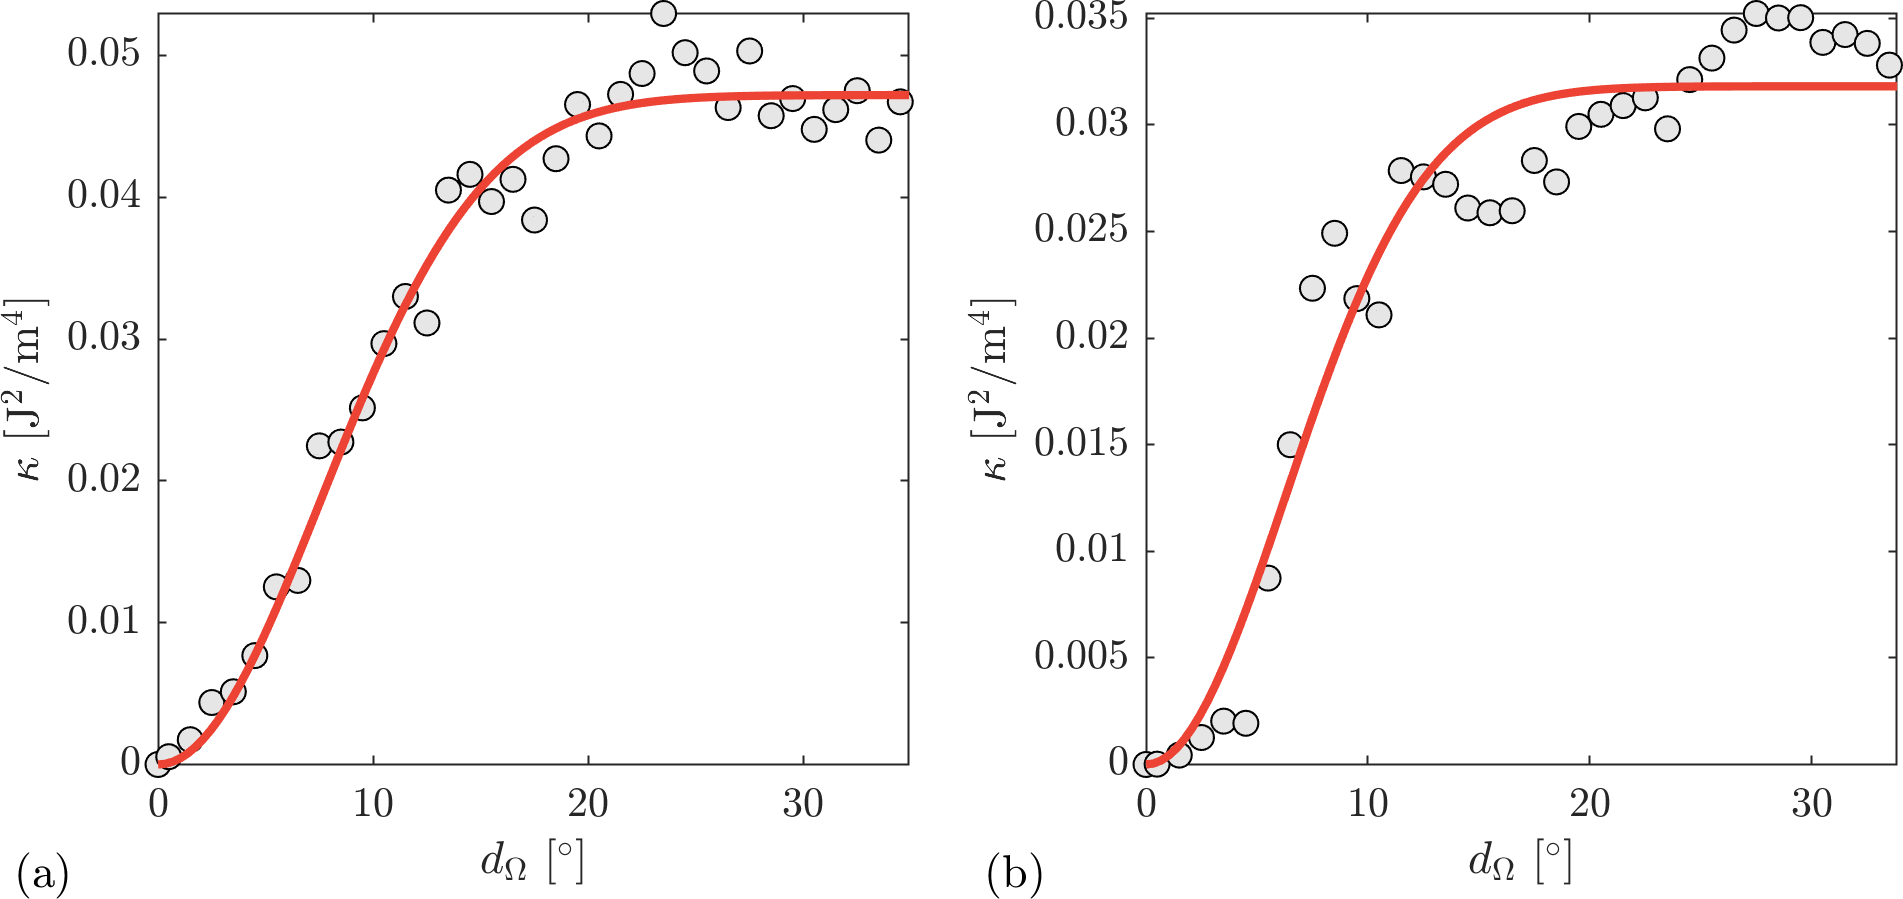
\includegraphics[scale=0.75]{figures/GlobalCorrelationLengthVariograms.png}
% 	    \caption{Empirical semivariograms (markers) for the (a) Ni and (b) Fe datasets. Solid lines show the fits of the analytical semivariogram models (\cref{eq:analyticalsemivariogrammodel}).}
% 	    \label{fig:globalvariogramfits}
% 	\end{figure*}
	
% 	One of the most fundamental observations comes from the shape of the empirical semivariograms. As mentioned in \cref{sec:methods:correlation}, there are a wide variety of kernels that could be candidates for modeling correlations in different systems. Different kernels are used to capture different types of correlations, and each has a characteristic signature that can be observed in the semivariogram. For example, when a system exhibits exponential-type correlations, the semivariogram manifests this in the form of an exponential convergence towards an asymptotic constant value at long-distances. Linear and power-type correlations manifest an absence of a long-distance plateau. In the present system, there is a clear change in concavity in the semivariogram, this is a signature of correlations that are Gaussian in nature. Thus, we find that \gls{gb} energy correlations in these systems are Gaussian, and should therefore be modeled using Gaussian kernels.
	
	In addition to the correlation length estimates obtained via the semivariogram method, we also computed correlation length estimates using the gradient-based \texttt{fitrgp()} method described in \cref{sec:methods:correlation}.
	
	To better understand the \gls{gpr} models that were trained on the \gls{gbe} data, we also interrogated their correlation lengths (as opposed to the input data only). This was done by the semivariogram method, with the \glspl{gbe} ($E\left(x_i\right)$ and $E\left(x_j\right)$ in \cref{eq:semivariogram}) given by the \gls{gpr} model (which is the mean of a collection of posterior models). This was done in two ways: (1) by evaluating the posterior models at the same locations as the input data, and (2) by evaluating the posterior models at randomly selected points (replications of which facilitate uncertainty quantification). The correlation lengths obtained by all of these methods are summarized in \cref{tab:globalcorrelationlengths}.
	\begin{table*}[]
	    \centering
	    \caption{Correlation lengths obtained via semivariogram and gradient based approaches in units of \gls{gbo} distance (multiply by 2 to get tilt angle). For the semivariogram of the posterior mean model evaluated at random points, we used $10^3$ random points and repeated this process 10 times. The corresponding values in this table represent the mean $\pm$ one standard deviation of those 10 replicates.}
	    \label{tab:globalcorrelationlengths}
	    \begin{tabular}{l c c}
	    \toprule
	         & \multicolumn{2}{c}{$l: d_\Omega\ [{}^{\circ}]$} \\
	         \cline{2-3}
	         & Ni & Fe \rule{0pt}{2.6ex}\\
	         \midrule
	         Semivariogram (Input Data) & 7.5491 & 6.2665 \\
	         Semivariogram (Posterior Mean at Input Points) & 7.7316 & 7.5179 \\ 
	         Semivariogram (Posterior Mean at Random Points) & $8.8551 \pm 0.1970$ & $7.7082 \pm 0.1746$ \\
	         Gradient (Input Data) & 7.3995 & 8.3073 \\
	         \bottomrule
	    \end{tabular}
	\end{table*}
	
	For the Ni dataset, the input data exhibits a correlation length of about $7.5\ d_{\Omega}^{\circ}$ for both the semivariogram and gradient methods. For the Fe dataset, we observe $6.2665\ d_{\Omega}^{\circ}$ for the semivariogram method and $8.3073\ d_{\Omega}^{\circ}$ for the gradient method, the average of the two being $7.3\ d_{\Omega}^{\circ}$. Thus both datasets seem to have correlation lengths of about $7.5\ d_{\Omega}^{\circ}$. This is significant. For symmetric tilt GBs, the octonion distance metric corresponds to half of the difference in misorientation angles. That means that in the more traditional units of degrees of misorientation difference the observed correlation lengths are very close to $15^{\circ}$, which is the traditional low-angle \gls{gb} threshold. Thus, the traditional $15^{\circ}$ threshold appears to hold (on average) more generally than just for differentiating low- and high-angle GBs. Rather we find that on average, \glspl{gb} that are within $15^{\circ}$ ($7.5\ d_{\Omega}^{\circ}$) will have well correlated energies regardless of their misorientations or \gls{gb} planes (i.e. it is not restricted to symmetric tilt GBs, but holds across the entire \gls{gb} character space).
	
	The correlation lengths obtained by evaluating the \gls{gpr} models are similar to those obtained directly from the input data, but they are slightly larger, suggesting that \gls{gb} energies in the trained models are correlated over a slightly longer distance than the input data, though the difference is nearly negligible (about $1\ d_{\Omega}^{\circ}$ or less).
	
	Using the correlation lengths, $l$, obtained via the semivariogram of the input data, \cref{fig:correlationlengthvsrho} shows the length scale, $l'$, corresponding to an arbitrary user-specified correlation strength, $\rho$. The length scales over which \gls{gb} energies are correlated range from $l' = 0\ d_{\Omega}^{\circ}$ for perfect correlation ($\rho = 1$) to $l' \approx 23\ d_{\Omega}^{\circ}$ and $l' \approx 19\ d_{\Omega}^{\circ}$ for essentially\footnote{Technically the correlation does not go to exactly zero until the length scale is infinite. The values listed here are for a correlation of $\rho = 0.01$.} zero correlation in the Ni and Fe datasets, respectively.
	\begin{figure}
	    \centering
	    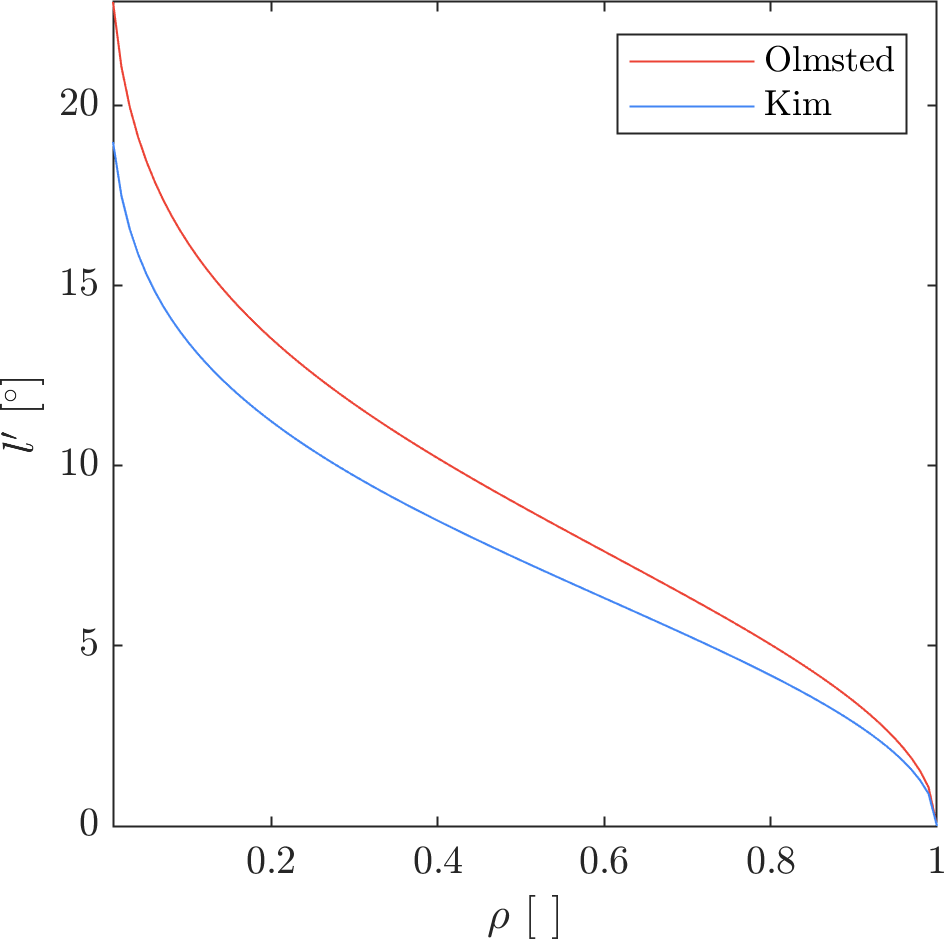
\includegraphics[scale=1]{figures/CorrelationLengthVsRho.png}
	    \caption{Global length scale of correlation, $l'$, in units of \gls{gbo} distance ($d_\Omega\ [{}^{\circ}]$) as a function of correlation strength, $\rho$, for the Ni (Olmsted) and Fe (Kim) datasets. Multiply \gls{gbo} distance by 2 to convert to tilt angle.}
	    \label{fig:correlationlengthvsrho}
	\end{figure}
	
	\Gls{gpr} facilitates numerically solving for correlation lengths (i.e. how similar properties are for similar crystallographic character), which are determined to be $\sim$\SIlist{7.4;8.3}{\degree} for the Ni and Fe datasets, respectively. If low noise is assumed for Ni, the correlation length drops to $\sim$2 degrees. See \cref{tab:resubloss-ni-pars} for \gls{gpr} parameters for each dataset. By contrast, if a \gls{gpr} model is trained on a large set of \num{50000} \glspl{gb} sampled from the \gls{brk} model, the numerically optimized correlation length is \SI{10.5}{\degree} suggesting that the \gls{brk} model imposes a-priori information that \glspl{gb} are more correlated than the data warrants. In other words, the \gls{brk} function is too smooth.
	
	\begin{table}[]
	\centering
	\caption{Fitted parameters for two \gls{gpr} models fitted to the 388 simulated Ni \glspl{gbe} by \citet{olmstedSurveyComputedGrain2009a} and fitted parameters for a \gls{gpr} model trained on 80\% of the Fe simulation data (\num{46883} \glspl{gb}). The first Ni model allows $\sigma$ to vary, whereas the second constrains $\sigma$ to be fixed. Mat., $\sigma_L$, $\sigma_F$, $\beta$, and $\sigma$ are the material (i.e. element), kernel length scale ($^\circ{}$), signal standard deviation ($J m^{-2}$), constant basis function ($J m^{-2}$), and input property standard deviation ($J m^{-2}$), respectively. %and a \gls{gpr} model trained on \num{50000} \gls{brk} model \glspl{gbe} are shown [NEED TO ADD].
	}
	\label{tab:resubloss-ni-pars}
	\csvautobooktabular[table head={\toprule Mat. & Fix $\sigma$ & $\sigma_L$ ($^\circ{}$) & $\sigma_F$ & $\beta$ & $\sigma$ \\\midrule}]{tables/resubloss-ni-pars.csv}
    \end{table}
    
    % 	\subsubsection{Global Correlation Length} \label{sec:discuss:correlation:global}
	The two simulation datasets have distinct differences from each other, as summarized in \cref{tab:sim-compare}.
	\begin{table}[htb!]
	    \centering
	    \caption{Comparison of Ni (\citet{olmstedSurveyComputedGrain2009}) and Fe (\citet{kimPhasefieldModeling3D2014}) \gls{ms} simulation datasets. The differences in noise-levels results from whether multiple initial starting configurations were probed in search of a globally minimized configuration as opposed to using a single metastable configuration. }
\label{tab:sim-compare}
        \csvautobooktabular{tables/sim-compare.csv}
	\end{table}
	
	Despite these differences in terms of noise, dataset size, and crystal symmetry, it is interesting to see that the correlation lengths within a \gls{vfz} are similar for the two datasets. Both are lower than the correlation lengths of \SI{10}{\degree} \cite{rohrerComparingCalculatedMeasured2010} and \SI{15}{\degree} \cite{olmstedSurveyComputedGrain2009} previously reported\footnote{Both of these lengths are based on results from \citet{olmstedSurveyComputedGrain2009}.} with respect to misorientation, and are about on par in terms of \gls{bp} normal owing to the fact that \gls{gbo} distances for tilt angles are half the value of tilt angles.
	
	It is reasonable to assume that the Ni data has low noise due to use of a global optimization strategy \cite{olmstedSurveyComputedGrain2009}; thus, the correlation length of $\sim$\SI{1.9}{\degree} after imposing the low-noise condition suggests that \textit{the Ni dataset may have an actual correlation length much smaller than previously reported.}
	
	By contrast, the correlation length of a \gls{gpr} model trained on many \gls{brk} \glspl{gbe} remains relatively large at \SI{10.4}{\degree}. What does this suggest? The \gls{brk} model is smoothed more than the data warrants on its own. This has the following implications:
	\begin{enumerate}
	    \item More sophisticated methods are required which do not impose mistaken a-priori information about the correlation length\footnote{The a-priori information that the \gls{brk} model imposes is that correlation lengths within a \gls{mfz} or \gls{bpfz} hold for arbitrary paths through \gls{5dof} space and that moving from one subspace to another results in monotonic behavior. }. Instead, the data itself should suggest proper correlation lengths
	    \item Larger, low-noise datasets which span all \gls{5dof} are necessary to be confident in structure-property paths that are not restricted to a single \gls{mfz} or \gls{bpfz}
	\end{enumerate}
	
	We believe that the \gls{gpr} model within the \gls{vfz} framework meets the requirements of point \#1 and is capable of handling the ideal dataset proposed in point \#2.
	
	Some questions that remain are:
	\begin{itemize}
	    \item Does the similarity between correlation lengths for FCC and BCC extend to non-cubic crystal symmetries?
	    \item What are the differences in correlation length for other properties? (e.g. mobility)
	\end{itemize}
	%
	It is possible that the correlation length will increase with the size of the \glspl{vfz}, and we expect that the correlation length will depend on the property of interest.
	
    \subsubsection{Local Correlation Lengths} \label{sec:results:correlation:local}
    
    In addition to the global correlation lengths reported in \cref{sec:results:correlation:global}, we also investigated correlation length scales locally in the vicinity of certain low-$\Sigma$ GBs. This is accomplished by the same semivariogram process explained in \cref{sec:methods:correlation}, except that in \cref{eq:semivariogram} we consider only pairs of \glspl{gb} for which one of the \glspl{gb} is the particular \gls{gb} of interest (i.e. we fix one of the GBs). Because the resulting set of \gls{gb} pairs is smaller than in the global analysis, we use larger bins with a width of $2\ d_{\Omega}^{\circ}$ for the local empirical semivariograms.
    
    \Cref{fig:localvariogramsolmsted,fig:localvariogramskim} show the local empirical semivariograms for the Ni and Fe datasets respectively. Each panel shows the semivariogram centered at a different low-$\Sigma$ GB. While noisier than the global empirical semivariograms, reasonable fits were obtained for all except $\Sigma 5$ in the Ni dataset \cref{sec:supp:semivariogram:local}.
    
    % \begin{figure*}
    %     \centering
    %     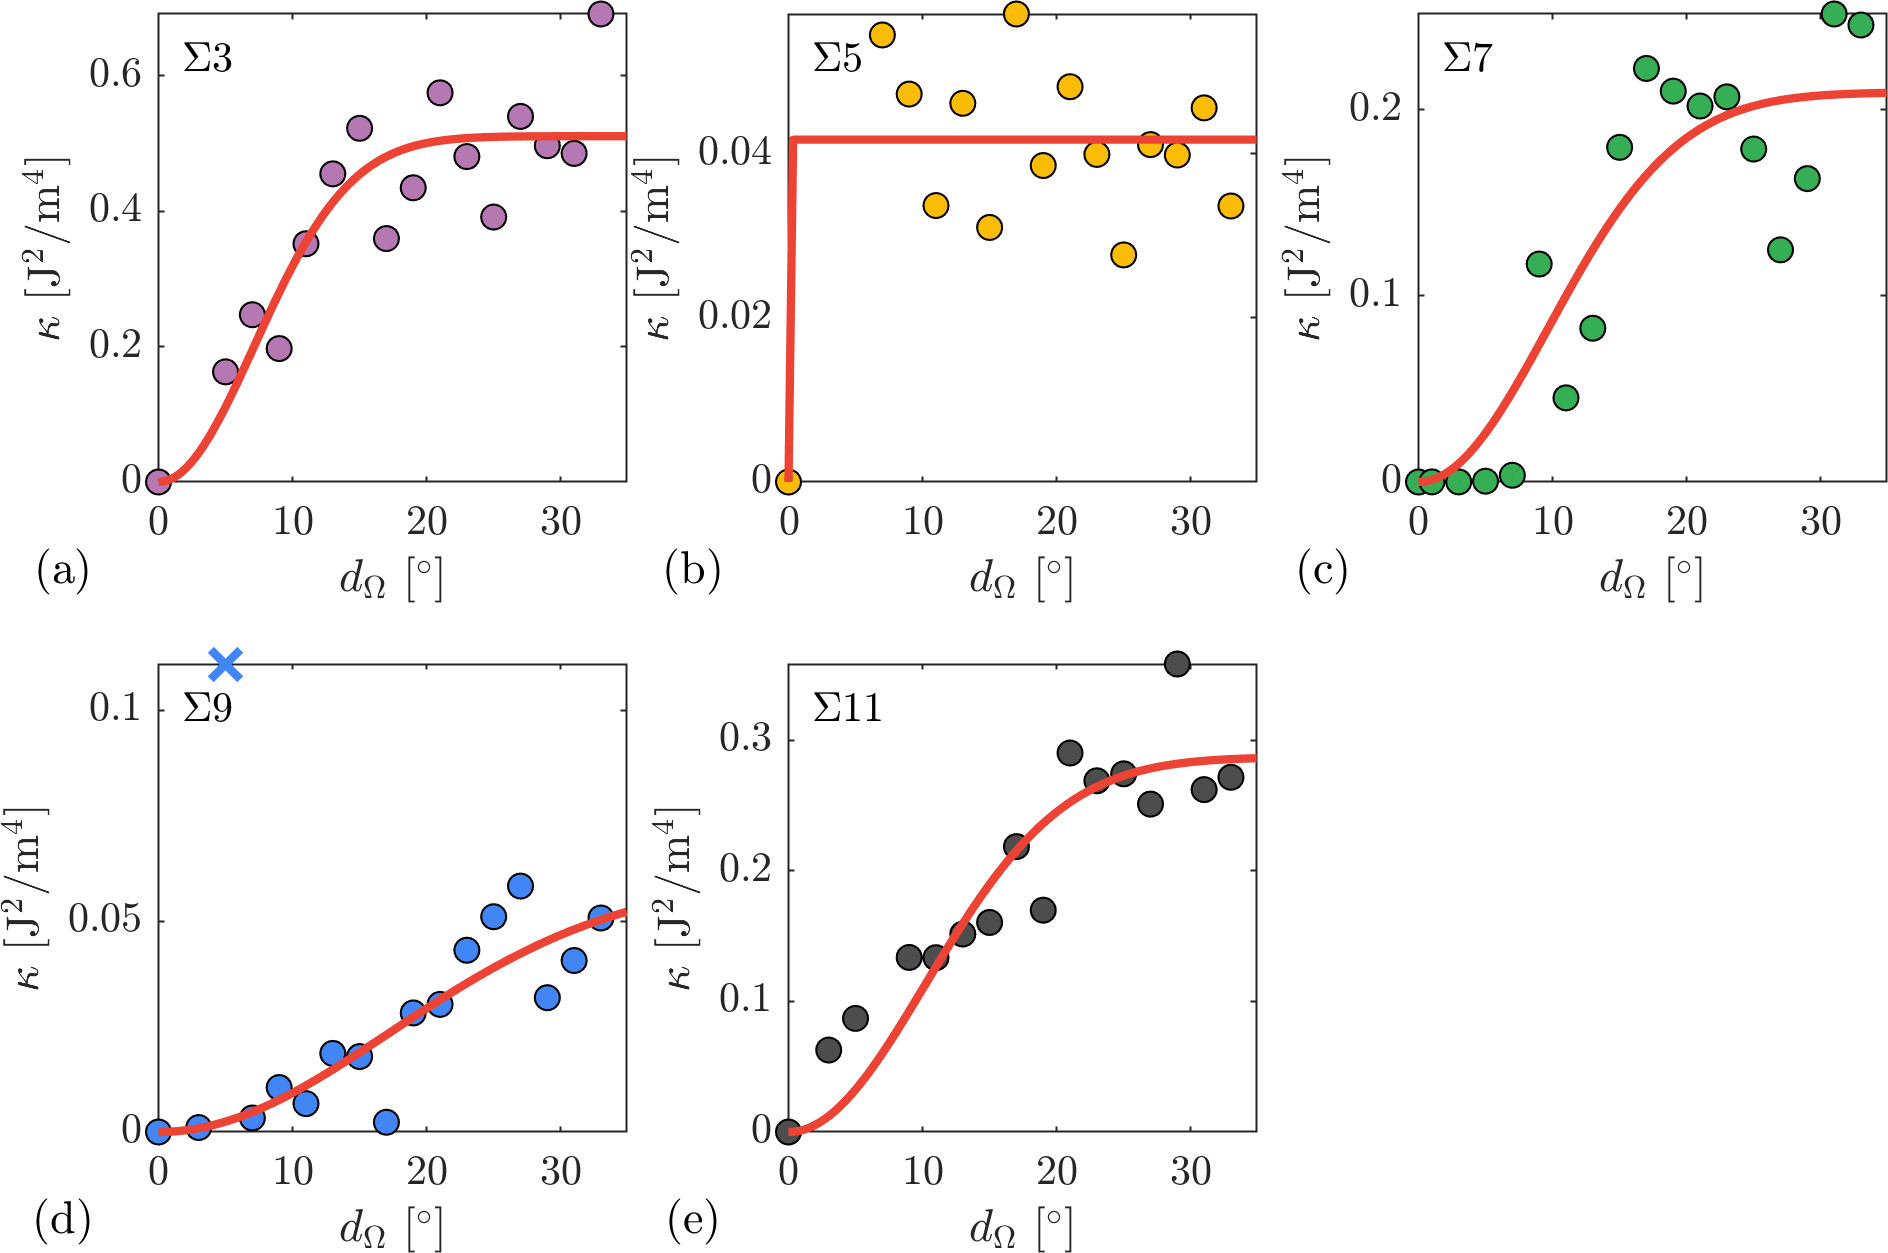
\includegraphics[scale=1]{figures/LocalCorrelationLengthVariogramsOlmsted.png}
    %     \caption{Local empirical semivariograms (markers), respectively centered at various low-$\Sigma$ \glspl{gb} for the Ni dataset. Solid lines show the fits of the analytical semivariogram models. In (d) the one point marked with an $\times$ was considered an outlier and was excluded from the fit.}
    %     \label{fig:localvariogramsolmsted}
    % \end{figure*}
    % \begin{figure*}
    %     \centering
    %     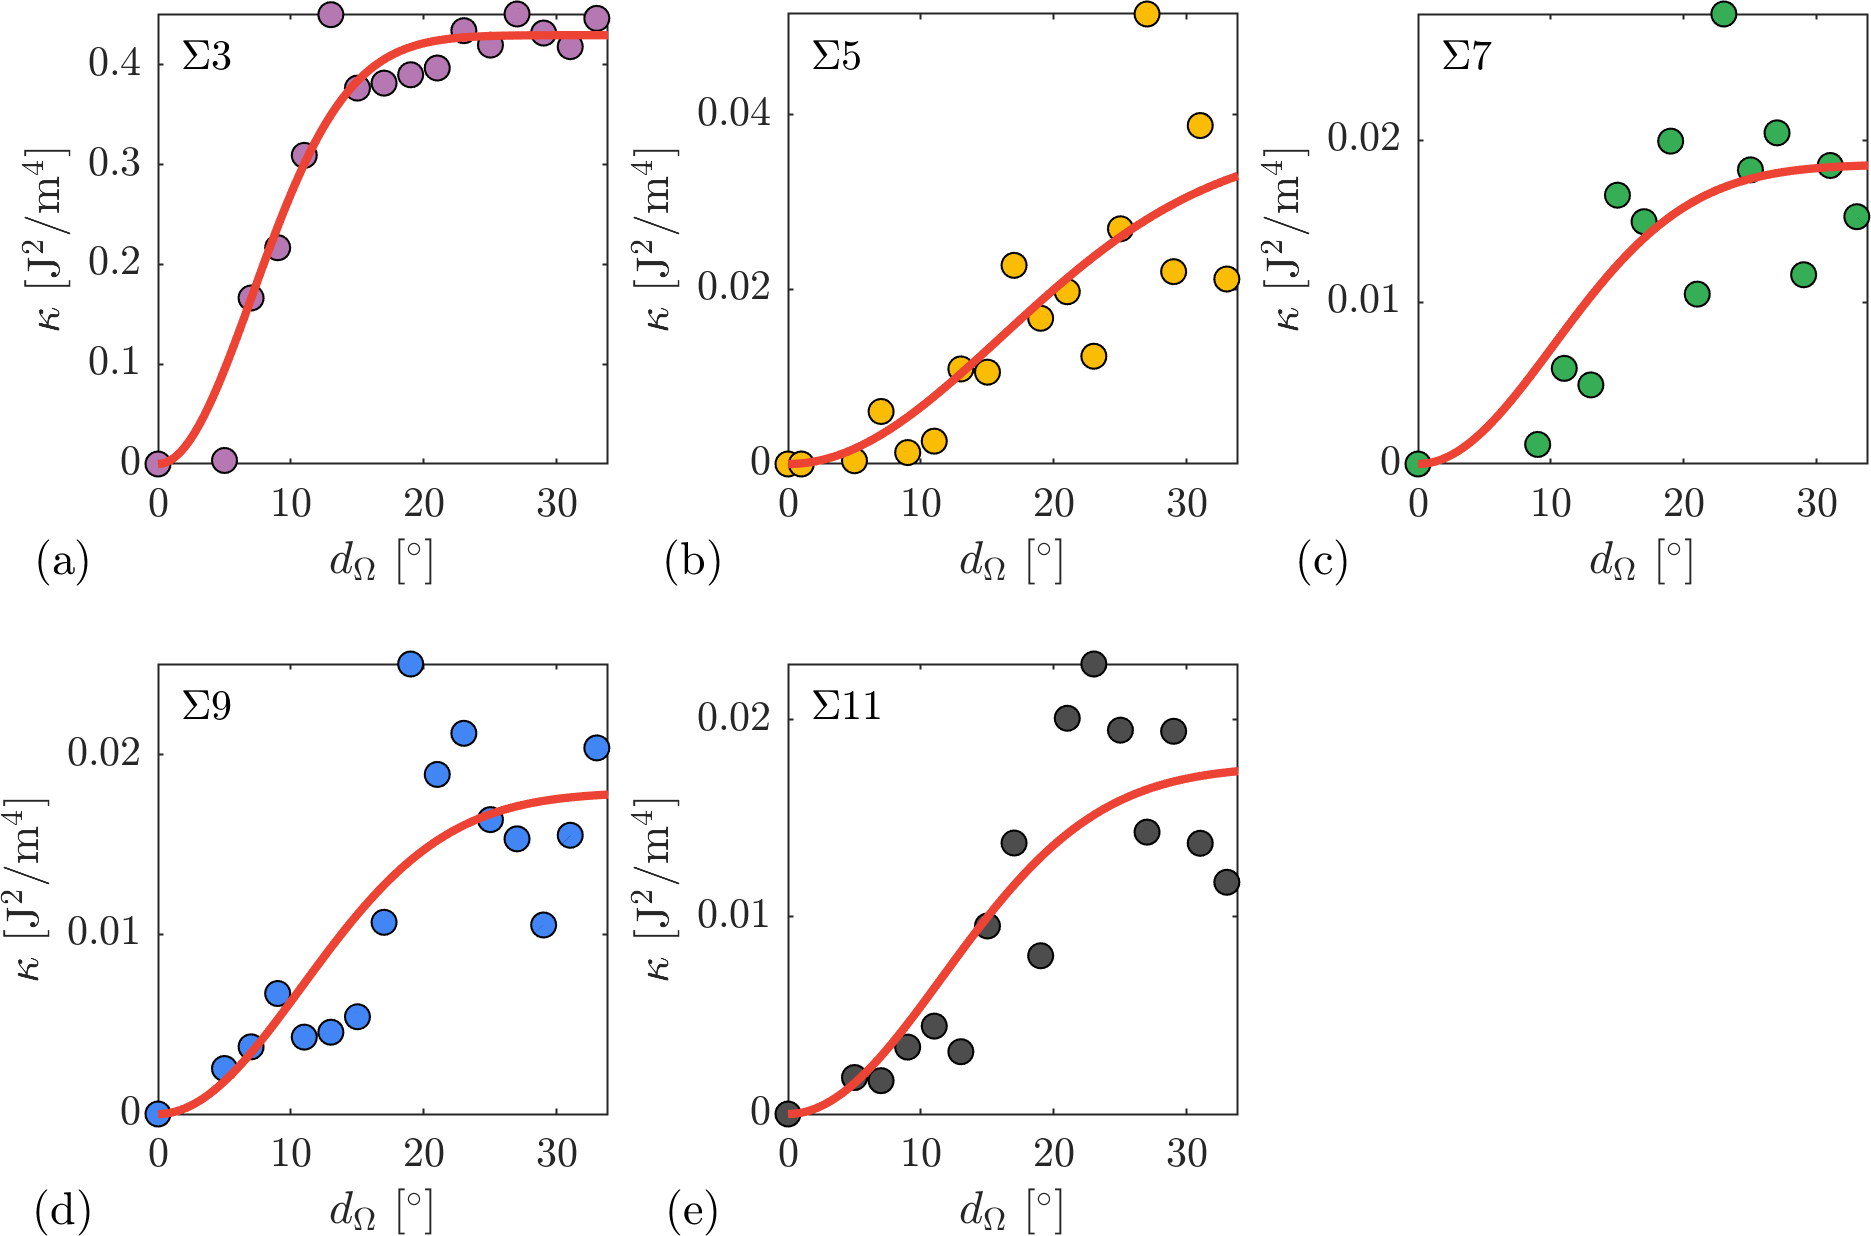
\includegraphics[scale=1]{figures/LocalCorrelationLengthVariogramsKim.png}
    %     \caption{Local empirical semivariograms (markers), respectively centered at various low-$\Sigma$ \glspl{gb} for the Fe dataset. Keys for which \glspl{gb} each of these correspond to in the original papers are given for Fe and Ni in \cref{tab:sigma-key-olmsted,tab:sigma-key-kim}, respectively. Solid lines show the fits of the analytical semivariogram models.}
    %     \label{fig:localvariogramskim}
    % \end{figure*}
    % The local empirical semivariograms are noisier than the global empirical semivariograms, likely due to considering fewer \gls{gb} pairs. Nevertheless, reasonable fits were obtained for most of the \glspl{gb} with the exception of the $\Sigma 5$ \gls{gb} in the Ni dataset. In many of the local semivariograms we again see the signature change in concavity suggesting that the local correlations in the vicinity of these \glspl{gb} are also Gaussian in nature. However, there are some exceptions where the nature of the correlations is more ambiguous. We anticipate that this ambiguity could be resolved with datasets that are either larger (compared to the Ni dataset) or having less noise (compared to the Fe dataset) than those considered here. However, the local empirical semivariograms seem to be generally consistent with Gaussian-type correlations.
    
    \Cref{tab:localcorrelationlengths} provides the correlation local lengths obtained for each of the low-$\Sigma$ \glspl{gb} for each of the datasets. The most noteworthy observation is that these correlation lengths are different from one another and different from the respective global correlation lengths. While the local correlation lengths for the $\Sigma 3$ \glspl{gb} are similar to the global values for both datasets, other \glspl{gb} have correlation lengths more than twice as large as the global correlation length (the $\Sigma9$ in the Ni dataset, and the $\Sigma 5$ in the Fe dataset). The fact that certain local correlation lengths differ from the global correlation length suggests that a non-stationary Gaussian kernel (which depends on both relative distance and absolute location) may be a more appropriate choice than the stationary Gaussian kernel (\cref{sec:supp:semivariogram:local}).
    \begin{table}[]
	    \centering
	    \caption{Local correlation lengths in the vicininty of specific low-$\Sigma$ GBs, obtained via the semivariogram method in units of octonion distance. The fit of the $\Sigma 5$ \gls{gb} for the Ni dataset was sufficiently poor that we do not report a corresponding correlation length.}
	    \label{tab:localcorrelationlengths}
	    \begin{tabular}{l d{2.4} d{2.4}}
	    \toprule
	         & \multicolumn{2}{c}{$l: d_\Omega\ [{}^{\circ}]$} \\
	         \cline{2-3}
	         & \multicolumn{1}{c}{Ni} & \multicolumn{1}{c}{Fe} \rule{0pt}{2.6ex}\\
	         \midrule
	         $\Sigma 3$ & 7.1460 & 7.0921 \\
	         $\Sigma 5$ & \multicolumn{1}{c}{---} & 16.0440 \\ 
	         $\Sigma 7$ & 9.6533 & 10.1493 \\
	         $\Sigma 9$ & 17.2601 & 10.7792 \\
	         $\Sigma 11$ & 10.2027 & 11.6011 \\
	         \bottomrule
	    \end{tabular}
	\end{table}
	
    % The traditional Gaussian kernel exhibits the property of stationarity, meaning that the covariance depends only on the distance between two points, not on their respective locations (i.e. $\mathbf{C}_{\mathbf{m}_0}\!\left(x_i,x_j\right) = \mathbf{C}_{\mathbf{m}_0}\!\left(d\left(x_i,x_j\right)\right)$). The use of a stationary kernel implies a prior assumption that there is a single global correlation length that applies everywhere. The fact that we observe significant variation in correlation length across the \gls{gb} character space suggests that it would be better to employ non-stationary kernels (this is why, when referring to the global correlation length results presented earlier, we were careful to say that the global correlation lengths hold "on average" across the space). In particular, due to the fact that the local semivariograms do seem to be generally consistent with Gaussian-type correlations, we suggest that the non-stationary version of the Gaussian kernel [REF] may be a reasonable choice. One additional potential benefit of employing non-stationary kernels might be improved resolution of cusps in the \gls{gb} energy landscape.
    
    These local correlation lengths facilitate an interesting comparison with the canonical Brandon criterion \cite{brandonStructureHighangleGrain1966a}. The Brandon criterion provides a threshold for the maximum angular deviation that can be accommodated by a \gls{csl} boundary before losing coincidence:
    \begin{equation}
        \Delta \theta = \theta_0 {\Sigma}^{-1/2}
        \label{eq:brandoncriterion}
    \end{equation}
    where $\Delta \theta$ is the angular deviation threshold, $\theta_0 = 15^{\circ}$ a constant corresponding to the low- to high-angle \gls{gb} threshold and $\Sigma$ is the reciprocal density of coincidence lattice points (i.e. the \gls{csl} number). The Brandon criterion predicts that amount of distortion that the \gls{gb} can accommodate (e.g. via introduction of \gls{gb} dislocations) before losing coincidence should \emph{decrease} with $\Sigma$ because the density of coincident sites decreases with $\Sigma$.
    
    In contrast, \cref{fig:brandoncriterioncomparison} shows that correlation lengths generally \emph{increase} with $\Sigma$. That is to say that in general there is a trend of \gls{gb} energies being correlated over longer length scales with increasing $\Sigma$. This seems reasonable since the deepest cusps in the \gls{gb} energy landscape (corresponding to small correlation lengths) tend to correspond to the lowest-$\Sigma$ GBs.
    \begin{figure}
        \centering
        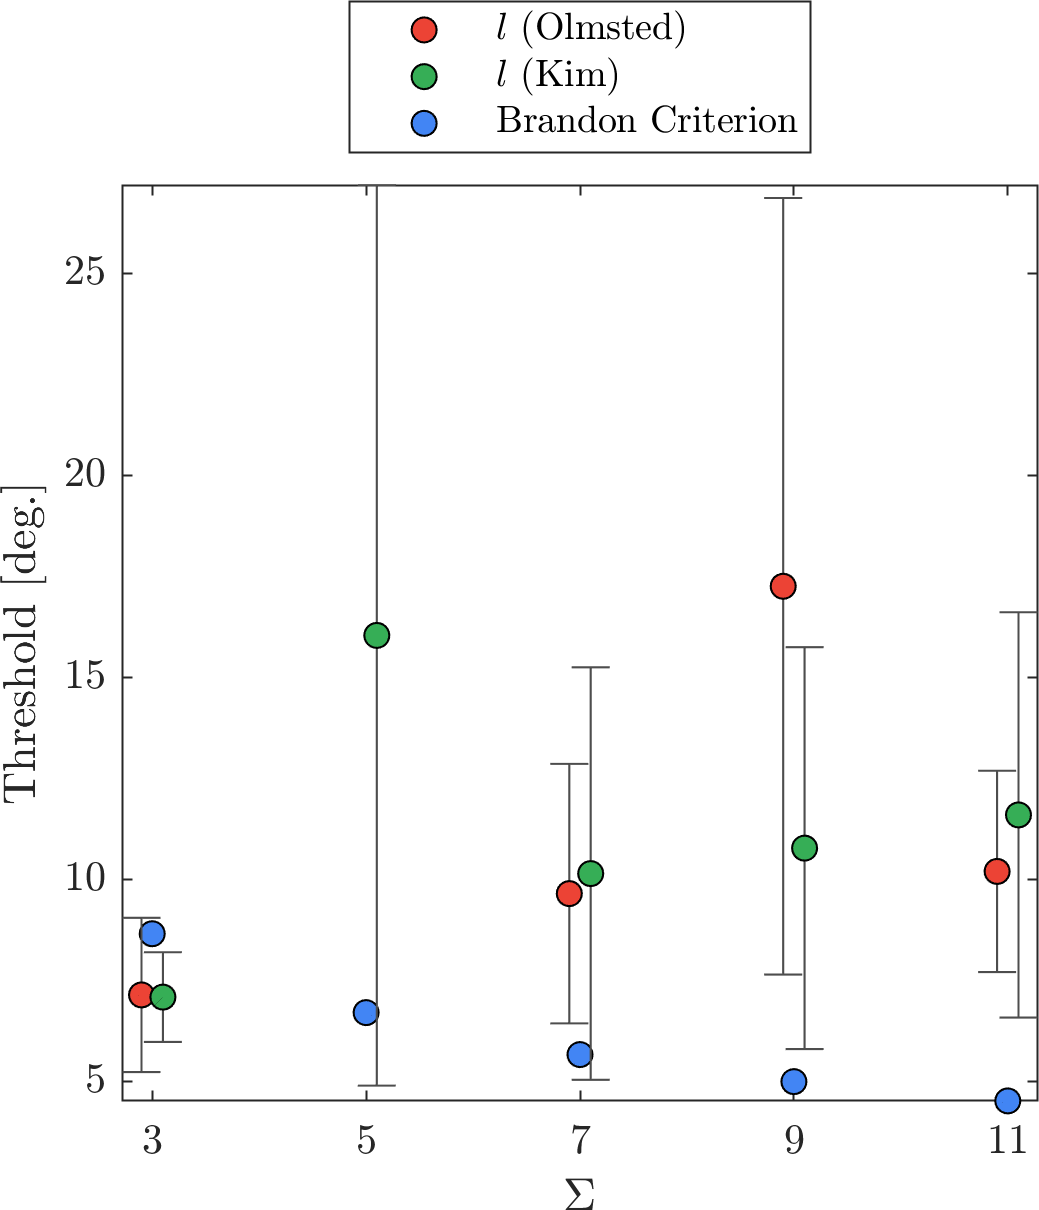
\includegraphics[scale=1]{figures/BrandonCriterionComparison.png}
        \caption{Comparison of the Brandon criterion \cite{brandonStructureHighangleGrain1966a} for low-$\Sigma$ \glspl{gb} (in units of ${}^{\circ}$) to the local correlation lengths obtained in this work (in units of $d_{\Omega}^{\circ}$). Conversion to consistent units would unnecessarily separate the data without changing the trends, and since we are most interested in the uniqueness of the trends rather than the numerical values themselves, we leave the values in their native units. Error bars indicate 95\% confidence intervals. There is no marker for the $\Sigma 5$ \gls{gb} in the Ni (Olmsted) dataset because of the failure of the fit discussed above.}
        \label{fig:brandoncriterioncomparison}
    \end{figure}
    This suggests that while strict coincidence may indeed be lost over smaller crystallographic deviations with increasing $\Sigma$, \gls{gb} energies seem to be relatively insensitive to this loss of coincidence and instead seem to be increasingly correlated over larger length scales. This may also imply that the \gls{csl} model becomes decreasingly relevant for predicting \gls{gb} energy as $\Sigma$ increases \cite{kingWhatDoesIt2006}.

	\subsubsection{Density and Distribution of Points} \label{sec:results:density}
	
	\Cref{fig:nndist-vs-setsize} illustrates how the \gls{vfzgbo} average \gls{nn} distance varies with the cardinality of the set (i.e. number of random \glspl{vfzgbo} in the set). The average \gls{nn} distance (over approximately 70 trials) of set sizes between \num{100} and \num{50000} between \SI{10.7175 \pm 0.3684}{\degree} and \SI{2.6479 \pm 0.2254}{\degree}, respectively. Additionally, a curve fit is given in the range of \num{388} to \num{50000}. For a specific \num{50000} \gls{vfzgbo} set, the \gls{nn} \gls{gbo} distance is \SI{\nnomega{}}{\degree} (\cref{fig:nnhist-knn-50000}a) while the average 100-th \gls{nn} distance is within \SI{10}{\degree} (\cref{fig:nnhist-knn-50000}b).
	
	\begin{figure*}
		\centering
		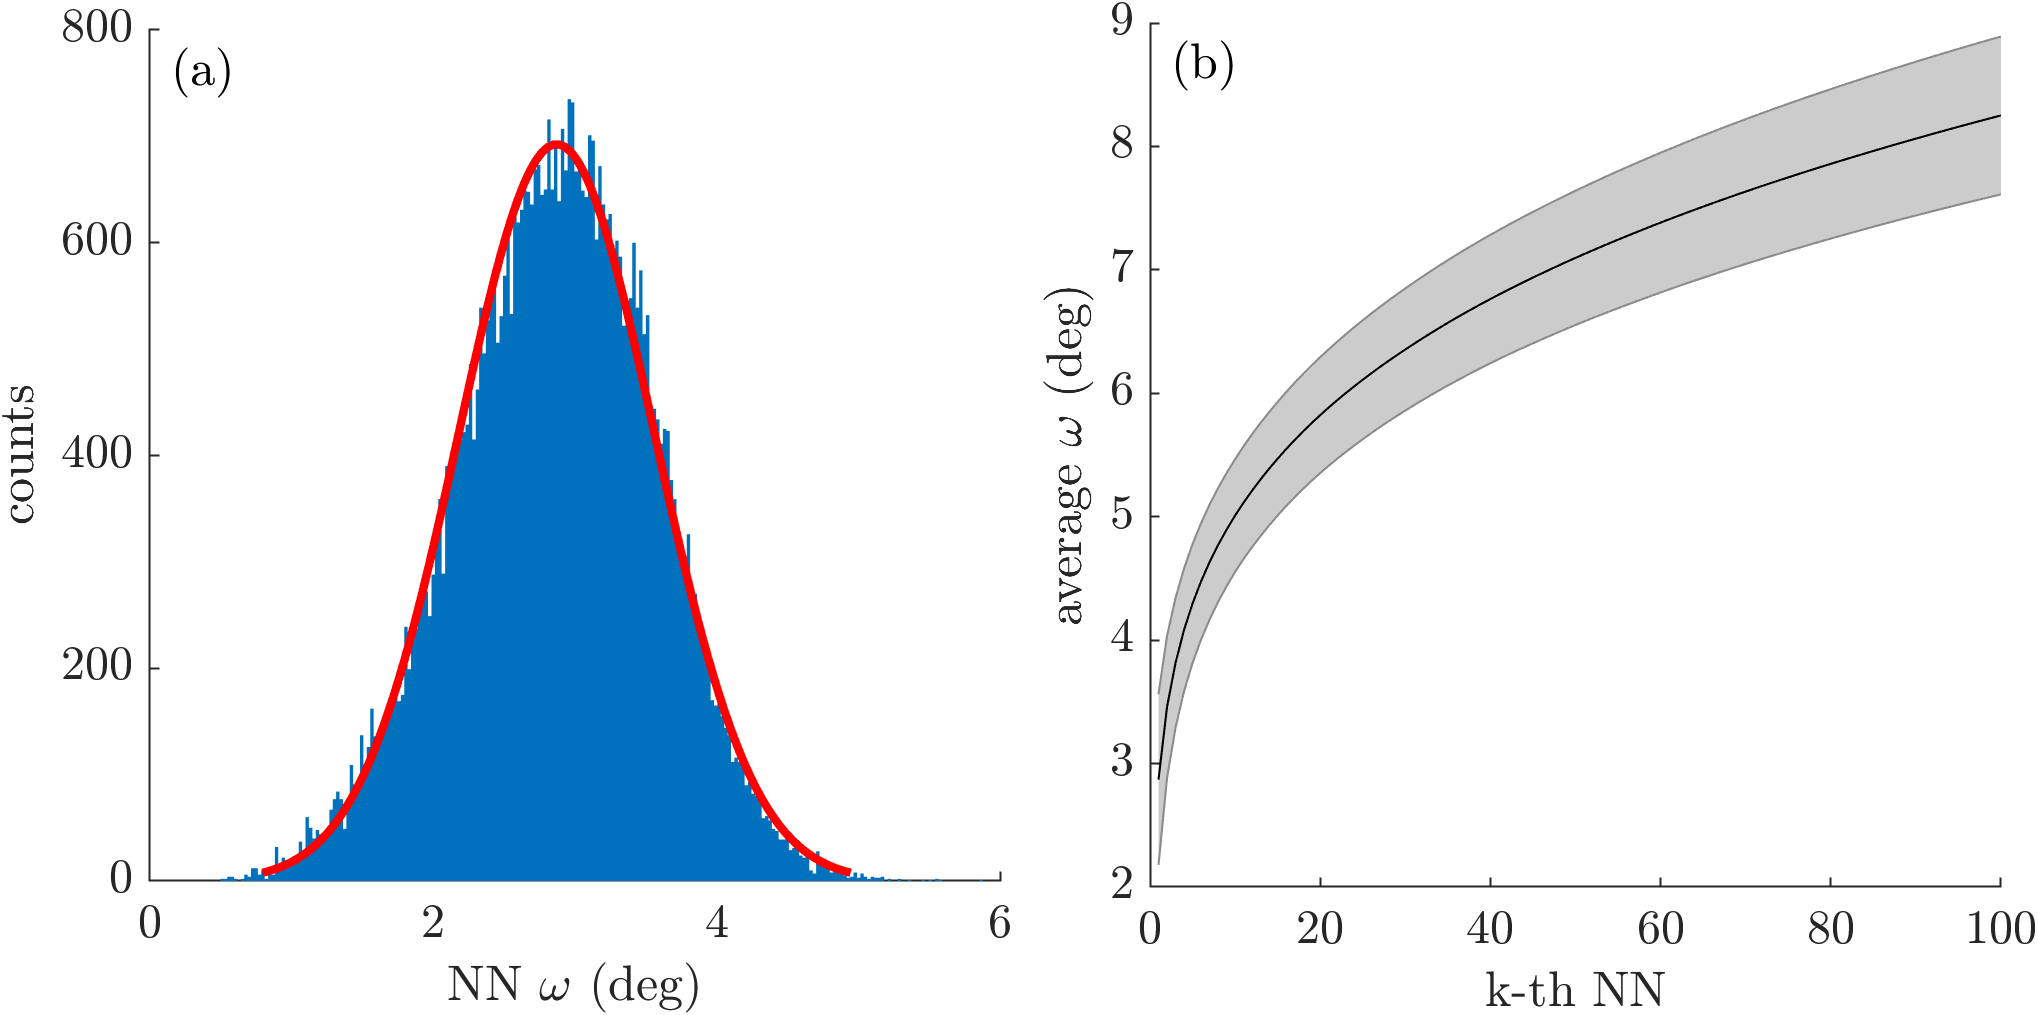
\includegraphics[scale=1]{nnhist-knn-50000.png}
		\caption{(a) Histogram of \gls{nn} \gls{gbo} distances ($\omega$) in a \gls{vfzgbo} set of \num{50000} points. The average \gls{nn} distance was \SI{\nnomega}{\degree}. (b) The average k-th nearest neighbor distances demonstrate that \glspl{nn} up to the $\sim$\num{10}-th \gls{nn} fall within a tolerance of $\sim$\SI{5}{\degree}. Standard deviation uncertainty bars using approximately 10 trial runs are also shown. }
		\label{fig:nnhist-knn-50000}
	\end{figure*}
	
	How large is the local region of influence for a \gls{5dof} interpolation model? These \gls{nn} distances give context to this question: if \num{50000} \glspl{gb} are randomly sampled, then on average, these \glspl{gb} are \SI{2.6479 \pm 0.2254}{\degree} apart from their \gls{nn}. In the context of correlation lengths of $\sim$\num{7}$-$\SI{8}{\degree} (\cref{sec:results:correlation:global}), a random set of at least $\sim$\num{10000} \glspl{gb} is required to reach a reasonable goal of half the correlation length (i.e. to have a reasonably performing structure-property model). By contrast, A set of \num{388} randomly sampled \glspl{gb} will yield average \gls{nn} distances of $\sim$\SI{7.5}{\degree}. The fact that this is approximately the same as the correlation lengths derived in this work suggest that this size of dataset is far too small. We demonstrate this via an example.
	
	Assume the property of a particular \gls{gb} which has been randomly sampled has never been measured before. What is available, however, is a set of property measurements for \num{388} other \glspl{gb}. Our model suggests that \gls{gb} which are further apart than $\sim$\SI{7.5}{\degree} can't reveal much information about each other. So, how many \glspl{gb} are in this local region of influence to be able to predict the property for the \gls{gb} of interest? The answer is only one \gls{gb}. To make matters worse, this \gls{gb} happens to be at the borderline distance of containing relevant information (closer is better).
	
	Correlation lengths can vary locally and are subject to some interpretation (\cref{sec:results:correlation:local}); however, it's clear that without knowing more, the property prediction of the \gls{gb} of interest might be OK, or it might be completely off. The \gls{brk} \cite{bulatovGrainBoundaryEnergy2014} model (which uses \num{388} \glspl{gb}) works around this limitation by imposing prior information: a "scaffolding" of \glspl{gb} at high-symmetry cusps is used, and it is assumed that the function varies monotonically from point to point everywhere else. For a well-studied property (\gls{gbe}) and a well-studied material system (FCC), this domain knowledge can be successfully baked in. But what if the property or material system is not so well understood? These are cases where the \gls{vfz} framework is especially useful.

	\begin{figure}
		\centering
		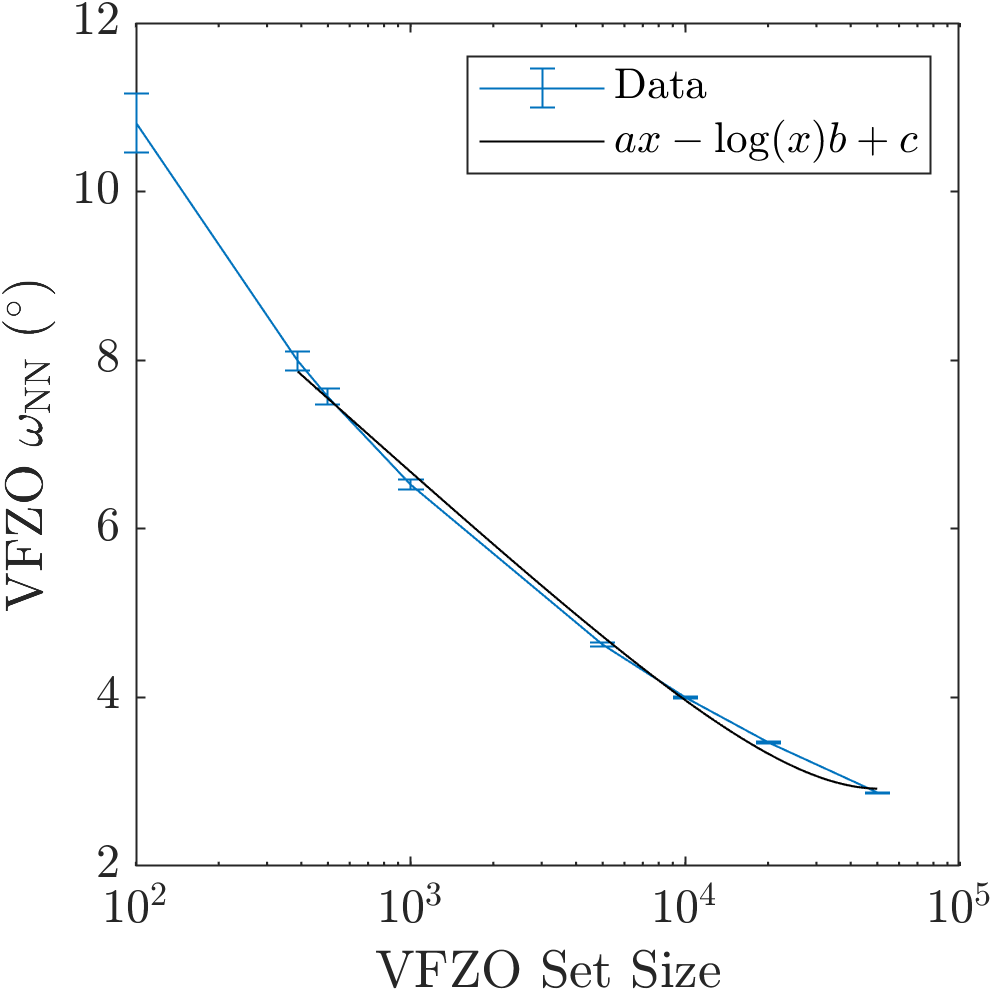
\includegraphics[scale=1]{nndist-vs-setsize.png}
		\caption{\Gls{nn} \gls{vfzgbo} ($\omega_{\text{NN}}$) distances ($^{\circ}$) versus \gls{vfzgbo} set size out of 70-80 random \gls{vfzgbo} sets per set size and a fit to $ax-\mathrm{log}(x)b+c$ where $a=2.5025\times10^{-5}$, $b=1.27396$, $c=15.4499$, $x$ represents set size, and $388 \leq x \leq 50000$.}
		\label{fig:nndist-vs-setsize}
	\end{figure}

	\subsection{Uncertainty of Noisy \glsentrytitlecase{ms}{long} Simulations} \label{sec:results:error}
	
	We analyze implications of results for a \gls{gprm} model developed for a noisy, Fe \gls{ms} simulation dataset.
	We find that:
	\begin{itemize}
		\item the model error is on par with the intrinsic uncertainty of the data (\cref{sec:results:lit:error})
		\item the predictions likely exhibit overprediction bias relative to the true minimum for a given \gls{gb} (\cref{sec:results:lit:overprediction})
		\item future availability of multiple metastable state \glspl{gbe} is anticipated to greatly improve the model performance (\cref{sec:results:lit:improve})
	\end{itemize}
	
	\subsubsection{Intrinsic Uncertainty} \label{sec:results:lit:error}
	We estimate the intrinsic uncertainty of an Fe \SI{0}{\kelvin} \gls{ms} simulation dataset to be \SIlist{0.06529;0.06190}{\joule\per\square\meter} depending on whether \gls{rmse} or \gls{mae} estimates are used, respectively. Minimum and maximum error was \SIlist{-0.2625;0.2625}{\joule\per\square\meter}, respectively.

	First, because only a single metastable state was used for each \gls{gbe} simulation, both the training and validation data are subject to noise, consistent with a wide lateral spread of predictions and the intrinsic uncertainty estimation (\cref{fig:kim-interp-degeneracy-results}). The Fe simulation dataset \gls{gprm} model gives lower \gls{rmse} (\SI{0.055035}{\joule\per\square\meter}) and \gls{mae} (\SI{0.039185}{\joule\per\square\meter}) than the uncertainty estimates. This indicates that the uncertainty itself is somewhat overestimated\footnote{The \outpt{} error of a model typically cannot be less than the noise of the \outpt{} data of a model even if the model is estimating the true \outpt{} values with better accuracy than the noise (which is very possible and even expected with \gls{gpr} models when the noise in the \inpt{} data is approximately Gaussian).}. The fact that both model and uncertainty metrics are relatively close and the prediction \cite{bairdFiveDegreeofFreedomPropertyUnderReview} and uncertainty parity plots (\cref{fig:kim-interp-degeneracy-results}b) are similar suggests that the model is performing well. It also suggests that further improvements in the model relative to the "true" values will be "hidden", i.e. they will probably not manifest as lower \gls{rmse} or \gls{mae} nor as more tightly distributed parity plots despite improving performance "behind the scenes".

    \subsubsection{Overprediction Bias} \label{sec:results:lit:overprediction}
	Next, given the theoretical existence of a true minimum \gls{gbe} for a given \gls{gb}, the predictions which were based on metastable \glspl{gbe} can be assumed to have an overprediction bias relative to the true minimum. On average, we expect this overprediction bias relative to the true minimum \gls{gbe} (rather than the most likely metastable state) may be on the order of a few hundred \SI{}{\milli\J\per\square\m} and may vary as a function of true minimum \gls{gbe}. In other words, the model obtained is probably an estimate of the most likely metastable \gls{gbe} rather than the true minimum \gls{gbe}. This is akin to saying that we obtain from this data a model that approximates the non-equilibrium, Stillinger quenched red curve of Figure 4(c1) in \cite{hanGrainboundaryMetastabilityIts2016}, not the minimum \gls{gbe} blue curve of the same chart. See \cite{hanGrainboundaryMetastabilityIts2016} for an in-depth treatment of equilibrium and metastable \gls{gbe}.

	\subsubsection{Improving on Existing Datasets} \label{sec:results:lit:improve}
	Finally, datasets where multiple metastable \glspl{gbe} (e.g. 3-10 repeats) are provided for each \gls{gb} will likely greatly improve the performance of the \gls{gpr} model in predicting either the most likely metastable \gls{gbe} (when all \glspl{gbe} are considered) or the true minimum \gls{gbe} (when only the minimum \gls{gbe} is considered for each \gls{gb}) and may even negate the need for a \gls{gprm} approach. Thus, it is suggested that, where feasible, future large-scale \gls{gb} bicrystal simulation studies report all property data for repeated trial runs rather than a single trial run or a single value from a set of trial runs. Ideally, data for the three additional microscopic \glspl{dof} for \glspl{gb} (which falls into the category of epistemic uncertainty in this work) would also be included. We believe it is likely that minimum energy paths (i.e. paths of steepest descent) in the \gls{gbe} landscape depend on both macroscopic and microscopic \glspl{dof} (in total, 8DOF) and could offer a more holistic view of \gls{gb} behavior that better mimics and explains experimental grain growth observations. Indeed, it has been experimentally observed that at least some \gls{gb} migration mechanisms involve structural transformations between equilibrium \glspl{gb} via metastable states \cite{weiDirectImagingAtomistic2021}.
	
	\subsection{\glsentrytitlecase{5dof}{short} Paths and \glsentrytitlecase{gb}{short} Behavior} \label{sec:results:paths}

% 	\subsubsection{Low Sigma \glsfmtshortpl{gb} }
	We analyze direct connections between low Sigma \glspl{gb} of interest to the materials science community. Using the set of 388 \glspl{gb} defined by \citet{olmstedSurveyComputedGrain2009}, we choose the $\Sigma5$, $\Sigma7$, $\Sigma9$, and $\Sigma11$ \glspl{gb} with the lowest \gls{gbe} out of the \citet{olmstedSurveyComputedGrain2009} Ni dataset\footnote{The IDs that correspond to each of the low-$\Sigma$ \glspl{gb} used for path visualization for the \citet{olmstedSurveyComputedGrain2009} and \citet{kimPhasefieldModeling3D2014} datasets are given in \cref{tab:sigma-key-olmsted} and \cref{tab:sigma-key-kim}, respectively. }; we then visualize direct paths as "tunnel" plots\footnote{Similar to traveling through a 1D tunnel while also looking at nearby points in the region close to the line in all directions.} in a \gls{vfz} between each of these and the global minimum $\Sigma3$ \gls{ct} \gls{gb} (\cref{fig:sigma-tunnels-olmsted}). This is performed for both the \gls{brk} and \gls{vfz}-\gls{gpr} models. Likewise, we perform \gls{gpr} for the Fe simulation dataset for \glspl{gb} of interest and also visualize these using tunnel plots (\cref{fig:sigma-tunnels-kim}).

	\begin{figure*}[!htb]
		\centering
		\begin{subfigure}[b]{0.4\textwidth}
			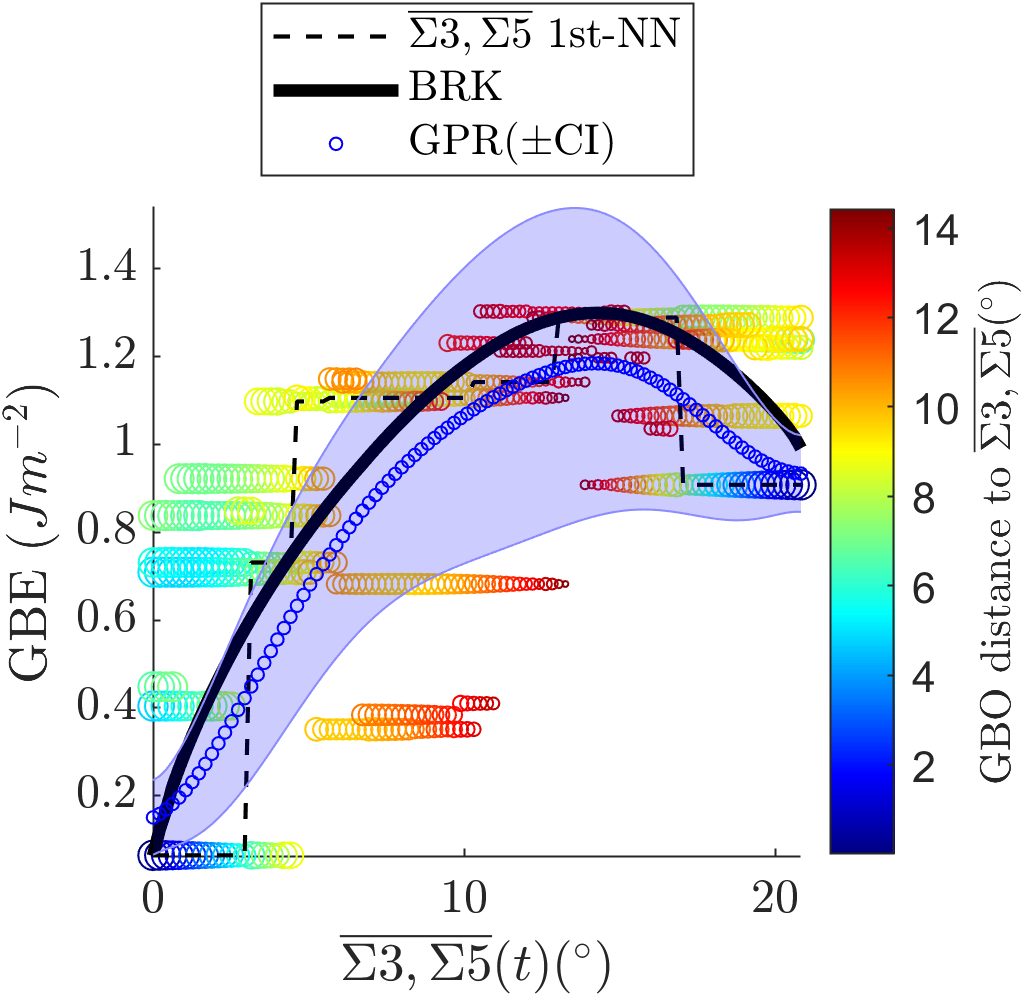
\includegraphics[width=\textwidth]{figures/tunnel-3-5-olmsted.png}
			\caption{}
			\label{fig:tunnel-3-5-olmsted}
		\end{subfigure}
% 		\hfill
		\begin{subfigure}[b]{0.4\textwidth}
			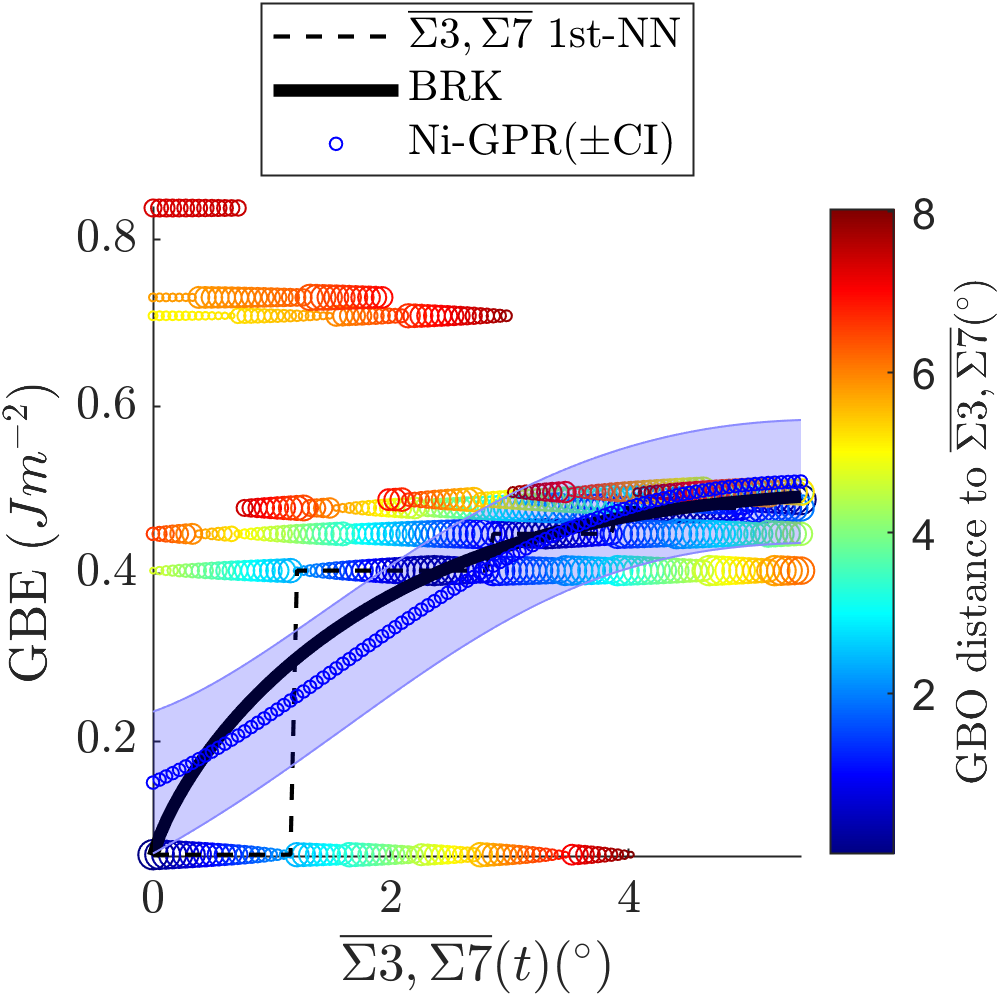
\includegraphics[width=\textwidth]{figures/tunnel-3-7-olmsted.png}
			\caption{}
			\label{fig:tunnel-3-7-olmsted}
		\end{subfigure}
		
		\begin{subfigure}[b]{0.4\textwidth}
			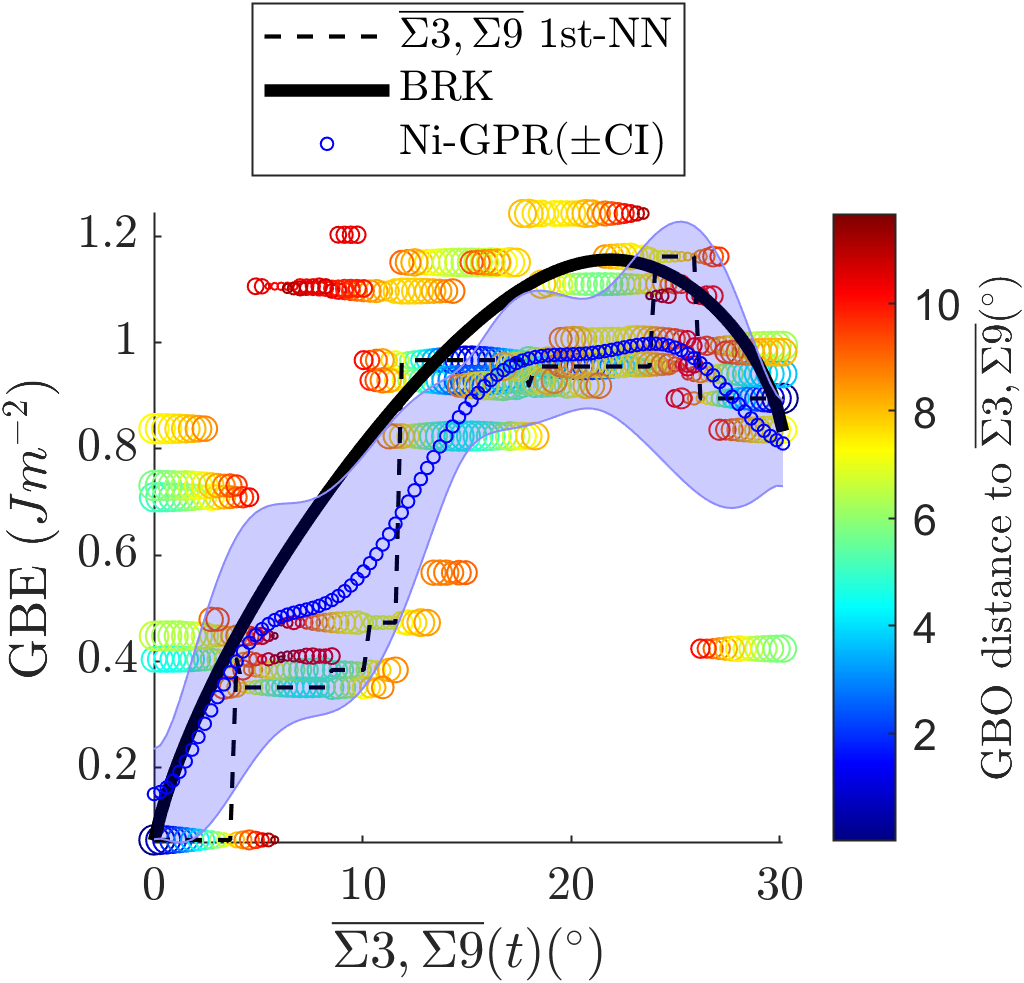
\includegraphics[width=\textwidth]{figures/tunnel-3-9-olmsted.png}
			\caption{}
			\label{fig:tunnel-3-9-olmsted}
		\end{subfigure}
% 		\hfill
		\begin{subfigure}[b]{0.4\textwidth}
			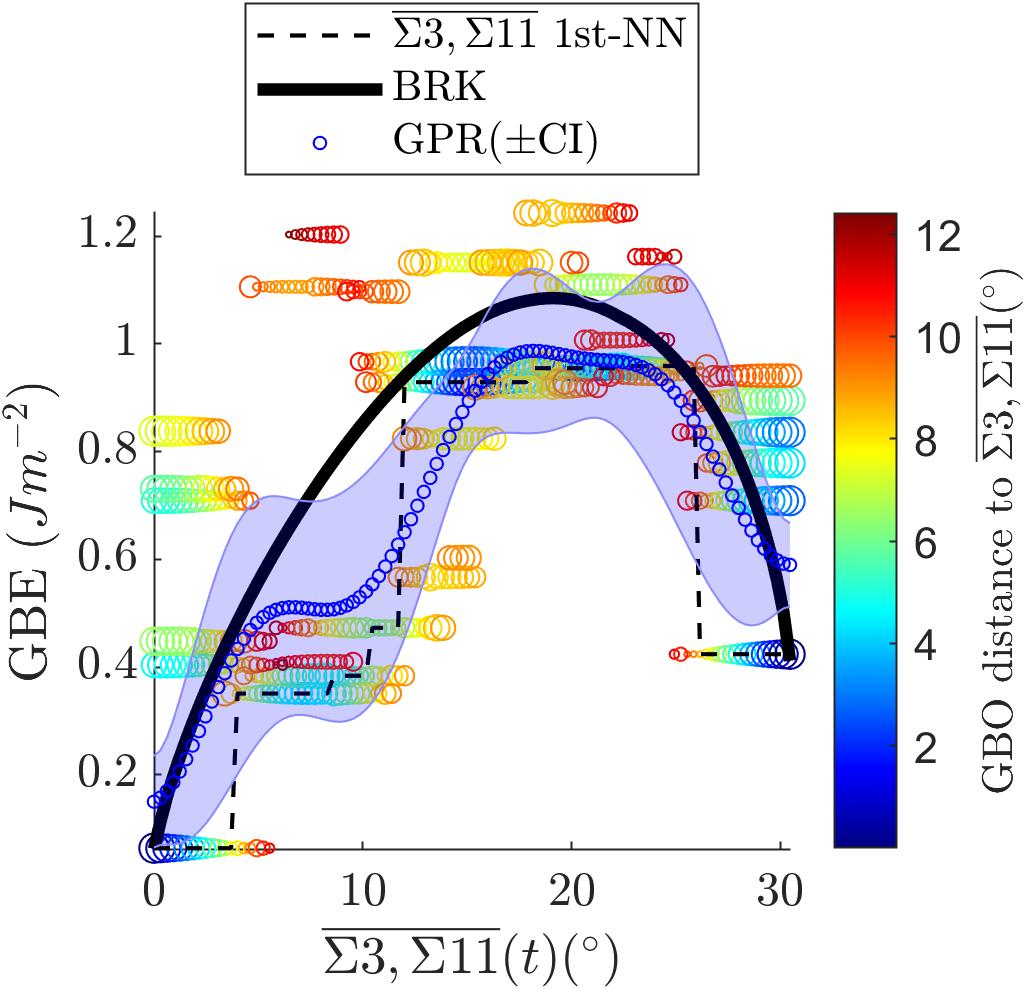
\includegraphics[width=\textwidth]{figures/tunnel-3-11-olmsted.png}
			\caption{}
			\label{fig:tunnel-3-11-olmsted}
		\end{subfigure}
		\caption{"Tunnel" plots of \glspl{gbe} along direct paths in a \gls{vfz} between the $\Sigma3$ \gls{ct} boundary and minimum \gls{gbe} (\subref*{fig:tunnel-3-5-olmsted}) $\Sigma5$, (\subref*{fig:tunnel-3-7-olmsted}) $\Sigma7$, (\subref*{fig:tunnel-3-9-olmsted}) $\Sigma9$, and (\subref*{fig:tunnel-3-11-olmsted}) $\Sigma11$ \glspl{gb} within the Ni \citet{olmstedSurveyComputedGrain2009} dataset. \Gls{gbe} values are plotted for the \gls{brk} and \gls{gpr} models which both used \citet{olmstedSurveyComputedGrain2009} as \inpt{} data. 95\% confidence intervals are plotted for the \gls{gpr} model. A "tunnel" plot is formed by calculating up to the 6th \glspl{nn} of the \inpt{} data relative to the direct path formed between two \glspl{gb}. The distances of the \glspl{nn} relative to the arc are used to both color and size the markers on the plot; \glspl{nn} which are closer to the arc are large, blue circles, whereas \glspl{nn} which are further from arc are small, red circles. Additionally, the 1st \gls{nn} path is plotted as a dashed line.}
		\label{fig:sigma-tunnels-olmsted}
	\end{figure*}
	
	\begin{figure*}[!htb]
		\centering
		\begin{subfigure}[b]{0.4\textwidth}
			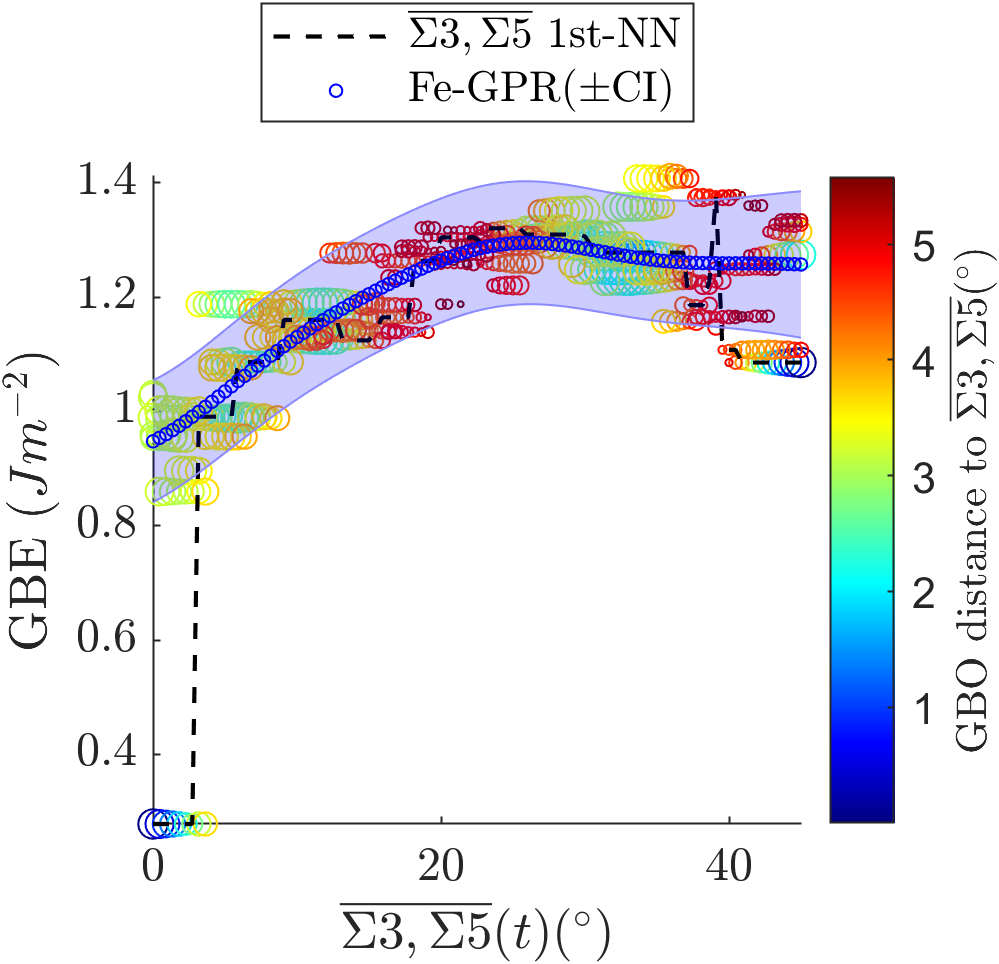
\includegraphics[width=\textwidth]{figures/tunnel-3-5-kim.png}
			\caption{}
			\label{fig:tunnel-3-5-kim}
		\end{subfigure}
% 		\hfill
		\begin{subfigure}[b]{0.4\textwidth}
			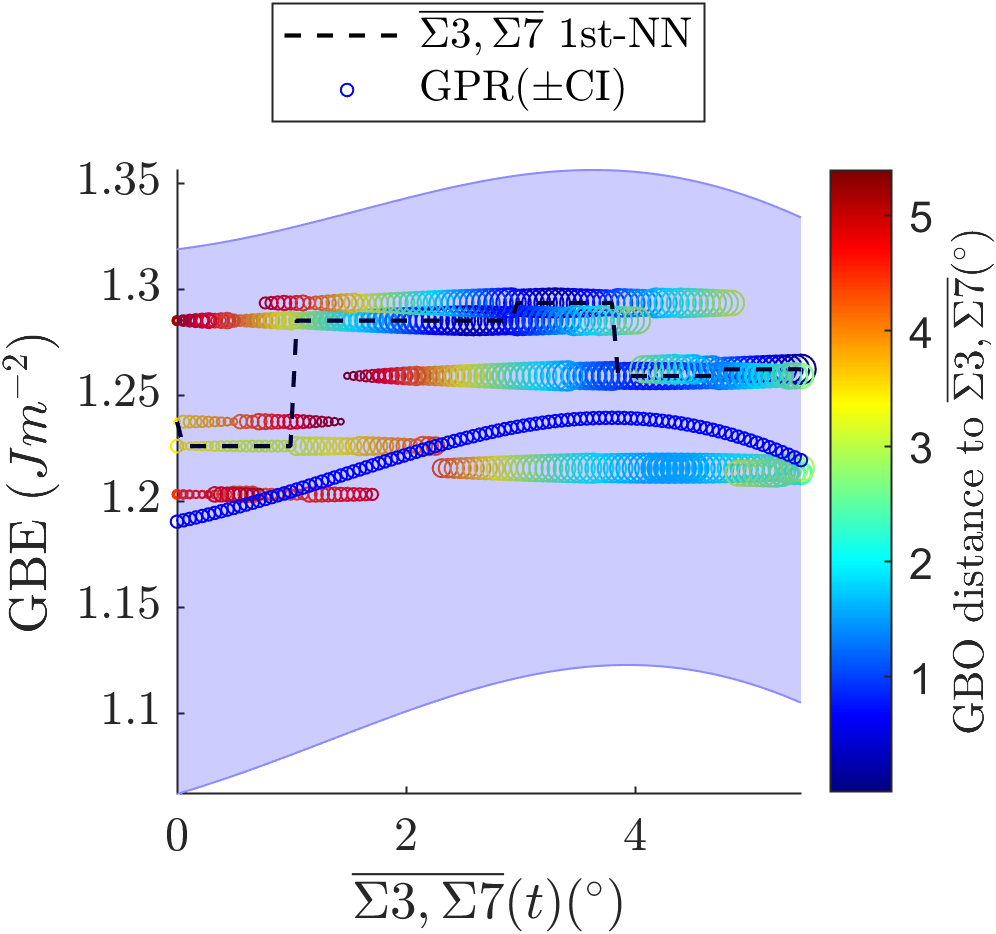
\includegraphics[width=\textwidth]{figures/tunnel-3-7-kim.png}
			\caption{}
			\label{fig:tunnel-3-7-kim}
		\end{subfigure}
		
		\begin{subfigure}[b]{0.4\textwidth}
			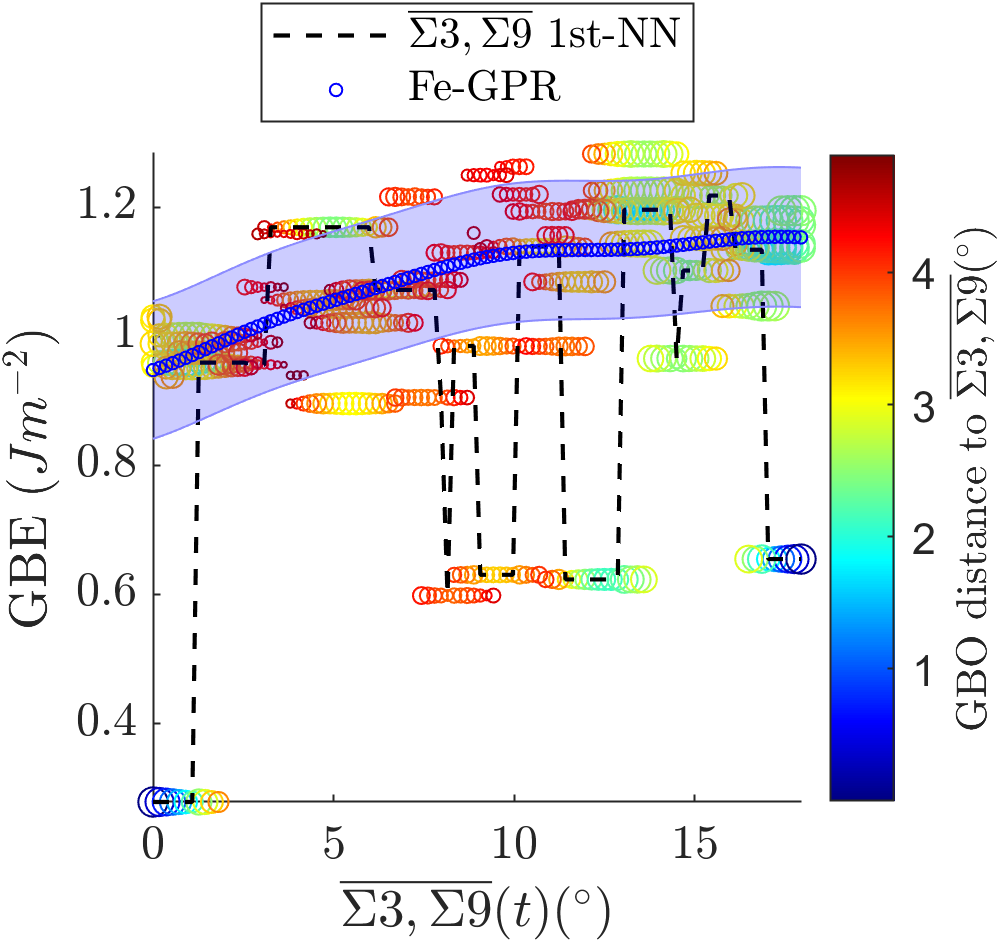
\includegraphics[width=\textwidth]{figures/tunnel-3-9-kim.png}
			\caption{}
			\label{fig:tunnel-3-9-kim}
		\end{subfigure}
% 		\hfill
		\begin{subfigure}[b]{0.4\textwidth}
			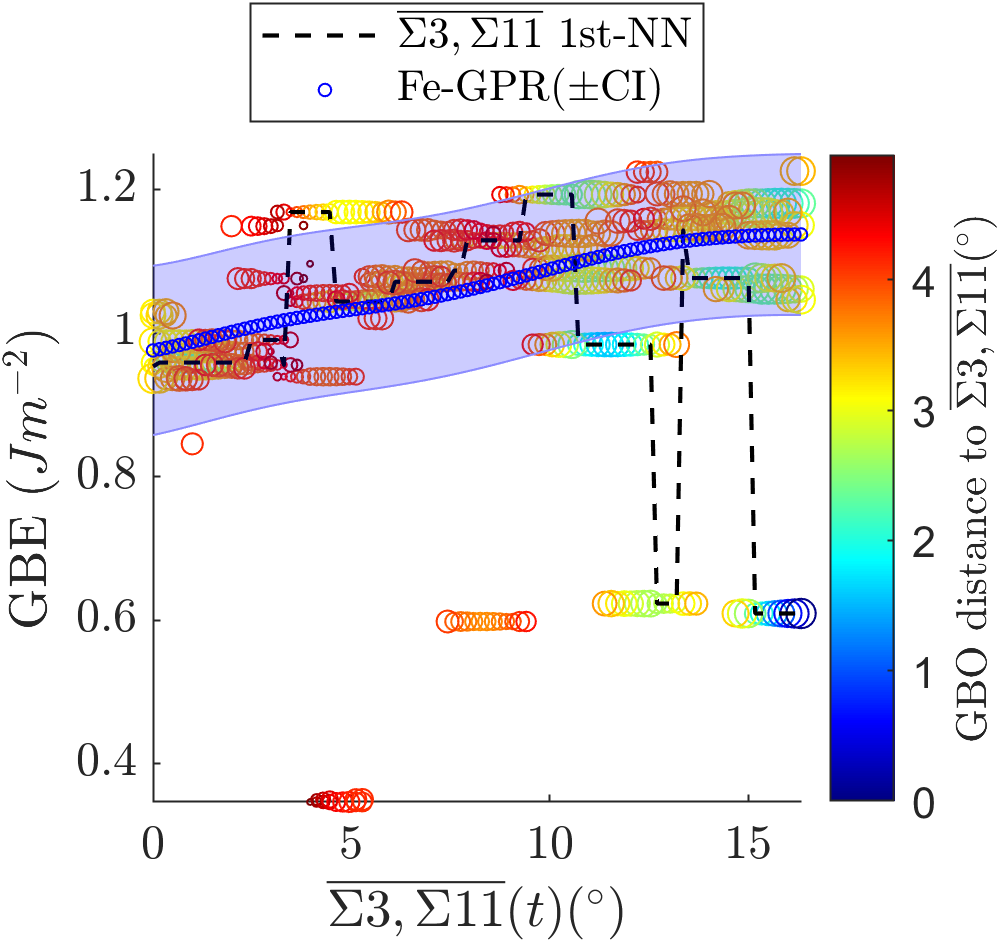
\includegraphics[width=\textwidth]{figures/tunnel-3-11-kim.png}
			\caption{}
			\label{fig:tunnel-3-11-kim}
		\end{subfigure}
		\caption{\Glspl{gbe} along direct paths in a \gls{vfz} between the minimum \gls{gbe} $\Sigma3$  and minimum \gls{gbe} (\subref*{fig:tunnel-3-5-kim}) $\Sigma5$, (\subref*{fig:tunnel-3-7-kim}) $\Sigma7$, (\subref*{fig:tunnel-3-9-kim}) $\Sigma9$, and (\subref*{fig:tunnel-3-11-kim}) $\Sigma11$ \glspl{gb} for the Fe \citet{kimPhasefieldModeling3D2014} dataset. A \gls{gpr} model trained on all \num{58604} Fe \citet{kimPhasefieldModeling3D2014} simulation datapoints was used. 95\% confidence intervals are plotted for the \gls{gpr} model. A "tunnel" plot is formed by calculating up to the 6th \glspl{nn} of the \inpt{} data relative to the direct path formed between two \glspl{gb}, similar to traveling through a 1D tunnel while also looking at nearby points in the region close to the line in all directions. The distances of the \glspl{nn} relative to the arc are used to both color and size the markers on the plot; \glspl{nn} which are closer to the arc are large, blue circles, whereas \glspl{nn} which are further from arc are small, red circles. Additionally, the 1st \gls{nn} path is plotted as a dashed line. }
		\label{fig:sigma-tunnels-kim}
	\end{figure*}
	
% 	 \subsection{\glsentrytitlecase{5dof}{short} Paths} \label{sec:discuss:path}
     For the \gls{gpr} model trained on the Ni \citet{olmstedSurveyComputedGrain2009} dataset, we observe that $\Sigma3$ and $\Sigma7$ are connected (i.e. no activation energy barrier) in \cref{fig:tunnel-3-7-olmsted} while the direct paths between $\Sigma3$ and $\Sigma5$, $\Sigma9$, $\Sigma11$ are separated by energy barriers (\cref{fig:tunnel-3-5-olmsted,fig:tunnel-3-9-olmsted,fig:tunnel-3-11-olmsted}). This indicates that for grain growth systems governed by \gls{gbe}, $\Sigma7$ \glspl{gb} may be more likely to transform into $\Sigma3$ \gls{ct} \glspl{gb}, whereas if $\Sigma5$, $\Sigma9$, or $\Sigma11$ transform into $\Sigma3$ \glspl{ct}, this will need to occur either by overcoming the activation energy or via paths through \gls{5dof} space other than the ones shown.  We note that while the \gls{gbe} path is direct with respect to crystallographic distances, the actual rotation of a grain is not a barrier-free transformation and requires energy to induce the crystallographic change [REF]. Thus, when grain rotation and other non-spontaneous atomic transitions are involved, the true energy path can be thought of as a signal of local energy barriers associated with atomic movement superimposed on the \gls{5dof} paths shown.
     
     The substantial vertical spread of the 1st-6th \glspl{nn} (colored, variable-size circles) are consistent with the fact that many points have distances on the order of \num{8}$-$\SI{14}{\degree} relative to the direct path between the two \glspl{gb}. For perspective, these distances are greater than the global correlation length of \SI{7.4}{\degree} (\cref{sec:results:correlation:global}), for which a higher proportion of distant points from the models are also distant crystallographically (small red and yellow circles). In other words, the local region of influence along the path is sparsely populated.
     
     For the \gls{gpr} model trained on the Fe \citet{kimPhasefieldModeling3D2014} dataset, the 1st \gls{nn} path and the \gls{gpr} path have substantial qualitative deviation from each other for $\overline{\Sigma3,\Sigma9}$ and $\overline{\Sigma3,\Sigma11}$ paths. While the \gls{gpr} model suggests that $\overline{\Sigma3,\Sigma11}$ are connected, the 1st \gls{nn} path suggests that there are local minima that are overestimated. Likewise, the 1st-6th \glspl{nn} (colored, variable-size circles) for $\overline{\Sigma3,\Sigma5}$ and $\overline{\Sigma3,\Sigma7}$ follow the general trend of the models. We observe that all \glspl{nn} distances up to the 6th \gls{nn} are less than $\sim$\SI{6}{\degree} from the paths of interest; this in turn is less than the global correlation length of \SI{8.3}{\degree} from \cref{sec:results:correlation:global} which indicates that local regions of influence along these paths in the Fe dataset are densely populated.
     
     By contrast, some \glspl{nn} have vastly different energies compared with the \gls{gpr} model. This is because the noise of the simulated \glspl{gbe} (\cref{sec:results:lit:error}) precludes the \gls{gpr} model from simultaneously resolving sharp transitions and maintaining smooth behavior elsewhere. This is one of the drawbacks of using a noisy dataset in a diverse space (some regions with sharp cusps, others with shallow hills and valleys) with a global smoothness (i.e. correlation) length.
	 %
	
	\subsection{Potential for Numerical Derivatives}
	\label{sec:results:deriv}
	
	 \Gls{gb} path visualizations in the \gls{vfz} framework suggest the ability to estimate numerical derivatives or gradients of \gls{gb} properties without being restricted to a \gls{gb} subspace (e.g. \gls{mfz} or \gls{bpfz}) which can be a useful mathematical construct for the \gls{gb} community. For example, steepest descent paths and all local \gls{gbe} minima can be estimated and used in grain growth simulations.
	
	Because distance overestimation exist in the \gls{vfz} framework, use of ensembled \gls{vfzgbo} interpolation or data augmentation may be necessary to mitigate discontinuity artifacts when crossing the exterior of a \gls{vfz} as discussed in \cref{sec:methods:framework}. Alternatively, the "excess" points in a gridded sampling can act as a type of data augmentation and help to address this issue. We plan to explore these topics in future work. \Cref{sec:supp:grid} contains further discussion of a gridded sampling approach.
	 
	\section{Conclusion} \label{sec:conclusion}
	We applied the \gls{vfz} framework to learning more about the nature of a \gls{5dof} \gls{fz}.

	The increase of distance computation throughput and the development of a \gls{5dof} \gls{vfz} with continuous coordinates enabled us to explore the nature of a \gls{5dof} \gls{fz}. We found that symmetrized \gls{nn} distances are Gaussian and plotted these as a function of set size. We determined the maximum principal component of a particular $O_h$ \gls{vfz} to be \dimOne{}.
	
	Other point groups (in particular those which are noncentrosymmetric) may give rise to differently shaped/larger \glspl{vfz} and for which the Euclidean approximation may need to be removed. It will be interesting to see the \gls{vfz} framework applied for other distance metrics (see \citet{morawiecDistancesGrainInterfaces2019} for a comprehensive summary of metrics).

	The interpolation errors for a Fe simulation dataset are on par with the intrinsic uncertainty of the dataset itself (\cref{sec:supp:kim-interp:quality}). Analysis of the \gls{gpr} fitting results indicates that the Ni and Fe simulation datasets have correlation lengths of \SIlist{8.3;7.4}{\degree}, respectively, but that when the Ni dataset is constrained to have low noise, the numerical correlation length drops to $\sim$\SI{1.9}{\degree}.
	%DISCUSS pairwise correlations & BRANDON'S CRITERIA, 2-4 sentences
	%
	Plotting of direct paths between low-Sigma \glspl{gb} of interest reveal that a $\Sigma$7 cusp has a monotonically decreasing path towards the \gls{ct} $\Sigma3$ cusp, whereas a $\Sigma5$, $\Sigma9$, and $\Sigma11$ cusps do not necessarily share this same type of monotonically decreasing path within a \gls{vfz}. We demonstrated that two cusps can be connected in \gls{5dof} space.
	
	In addition to its previous implementation for \gls{gb} property interpolation \cite{bairdFiveDegreeofFreedomPropertyUnderReview}, we anticipate the \gls{vfz} framework will continue to reveal important aspects of a \gls{5dof} \gls{fz} and inform us about material behavior especially with respect to grain growth and other large scale time-dependent or iterative processes.

	\section*{Acknowledgement}
	\label{sec:acknowledgement}
	
	The authors thank Ian Chesser, Toby Francis, Victoria Baird, Brandon Snow, and José Niño for useful discussions. This work was supported by the National Science Foundation under Grant No. 1610077. This work was supported in part through computational resources provided by Brigham Young University's Office of Research Computing.
	\section*{CRediT Statement}
	\textbf{Sterling Baird}: Conceptualization, Methodology, Software, Validation, Formal analysis, Investigation, Data Curation, Writing - Original Draft, Writing - Review \& Editing, Visualization. \textbf{Oliver Johnson}: Supervision, Project administration, Funding acquisition, Conceptualization, Writing - Review \& Editing. \textbf{David Fullwood}: Writing - Review \& Editing. \textbf{Eric Homer}: Funding acquisition, Writing - Review \& Editing

	
	% \appendix
\label{sec:app}
\section{Detailed Barycentric Interpolation Methods}
\setcounter{figure}{0}
\subsection{Triangulating a \glsentrytitlecase{vfz}{long} Mesh}
\label{app:bary-tri}

% Briefly (but clearly and explicitly) explain the steps of generating the cubochorically sampled GBs, converting them to octonions and then mapping all of them into the vfz. Then explain how you do the triangulation. This will require a few figures to show the process in 3D (i.e. generating a triangulation of a point cloud on a region of the surface of the 2-sphere).

% After random \glspl{vfzo} are obtained (\cref{sec:methods:rand}), % ...

In order to reduce the computational complexity of triangulating a high-dimensional mesh \cite{barberQuickhullAlgorithmConvex1996}, some simplifications are made. The degenerate dimension obtained from analytically minimizing $U(1)$ symmetry \cite{francisGeodesicOctonionMetric2019} is first removed via a rigid (i.e. distance- and angle-preserving) \gls{svd} transformation,
%to enable use of MATLAB's quickhull \cite{barberQuickhullAlgorithmConvex1996} implementations such as \texttt{delaunayn} and \texttt{convhulln}. Removal of the degenerate dimension is done via a rigid \gls{svd} transformation,
analogous to a Cartesian rotation and translation
%Thus, a set of octonions originally represented by 8D Cartesian coordinates are collapsed to a 7D Cartesian representation while preserving both distances and angles among the points
As a 3D Cartesian to 2D Cartesian analogue of this 8D Cartesian to 7D Cartesian transformation, we take a set . Next, this 7D Cartesian representation is projected onto a hyperplane tangent to the mean of the input points\footnote{This is \textit{not} a rigid transformation; however, it is sufficiently close to produce a high-quality triangulation in a \gls{vfz}.} (\cref{fig:bary-delaunay}b). The 7D Cartesian \glspl{gbo} undergo another rigid \gls{svd} transformation to 6D Cartesian (see 3D to 2D analogue in \cref{fig:bary-delaunay}c) for which a triangulation is computed via the quickhull algorithm \cite{barberQuickhullAlgorithmConvex1996} (see MATLAB function \texttt{delaunayn}).

\begin{figure}
    \centering
    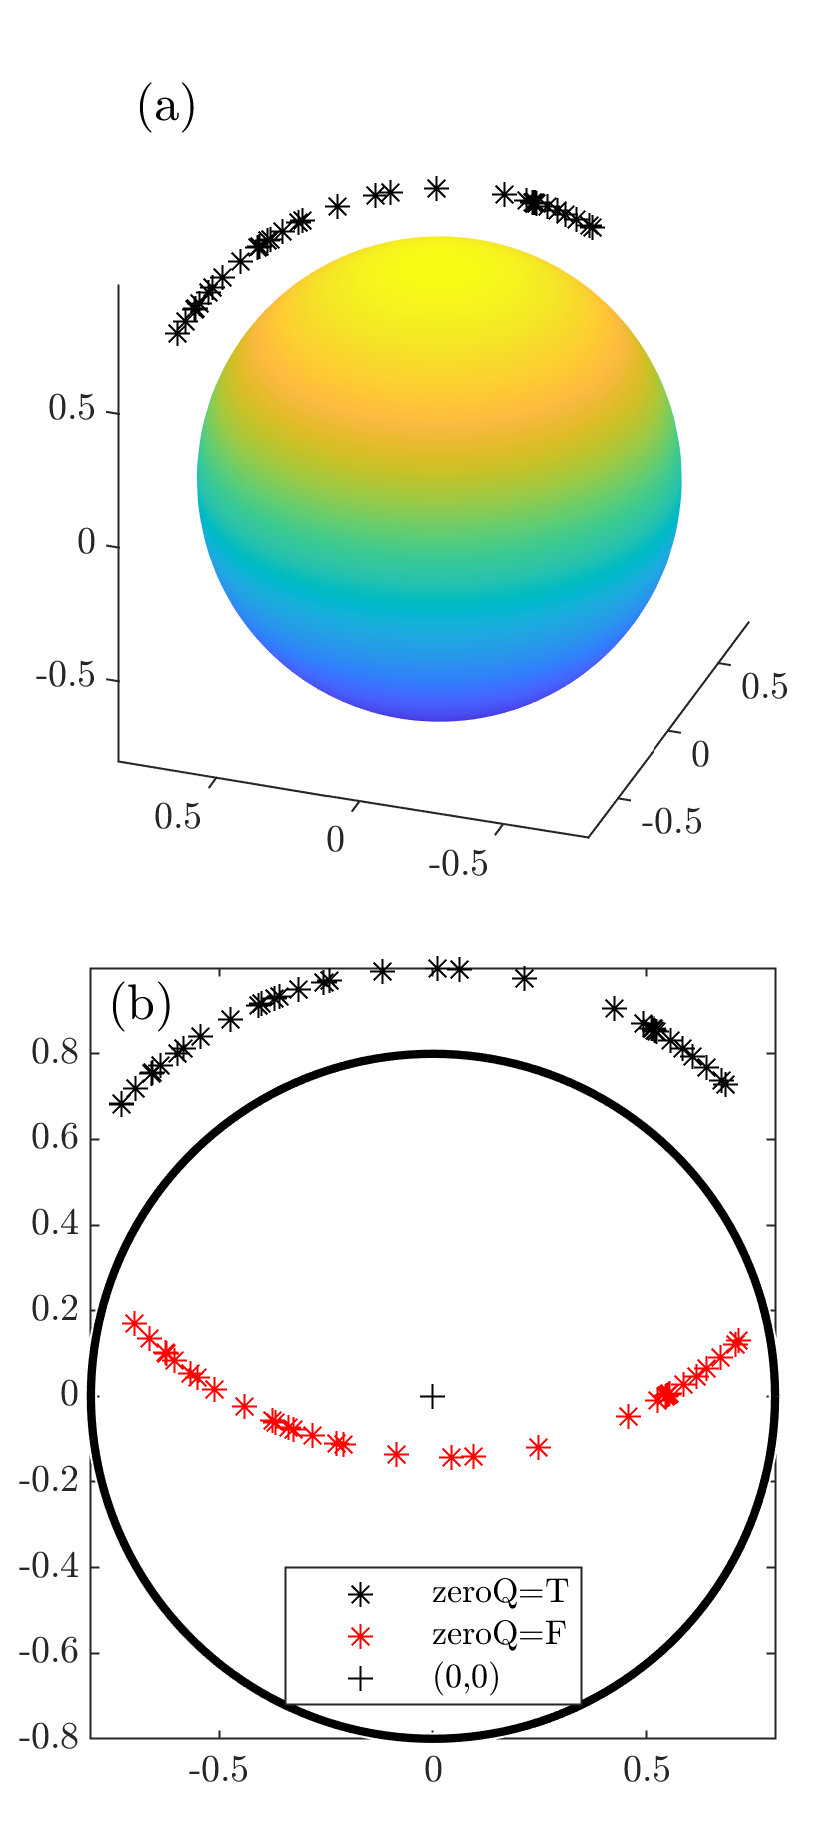
\includegraphics[scale=1]{bary-remove-deg.png}
    \caption{3D Cartesian to 2D Cartesian analogue of 8D Cartesian to 7D Cartesian degeneracy removal used in barycentric interpolation approach. Starting spherical arc points on surface of 2-sphere (a) and degenerate dimension removed via \acrlong{svd} transformation to 2D Cartesian (b) with either the origin (black plus) preserved (black asterisks, \texttt{zeroQ=T}) or ignored (red asterisks, \texttt{zeroQ=F}). The sphere (a) and circle (b) each have a radius of 0.8 and are used as a visualization aid only.}
    \label{fig:bary-remove-deg}
\end{figure}

Using a separate rigid \gls{svd} transformation from the triangulation, the original mesh and prediction \glspl{gbo} are simultaneously transformed from 8D Cartesian to 7D Cartesian. Because our \gls{svd} approach is rigid, the triangulation is then superimposed onto the newly transformed input points resulting in a 7D Cartesian \gls{vfz}.

\begin{figure}
    \centering
    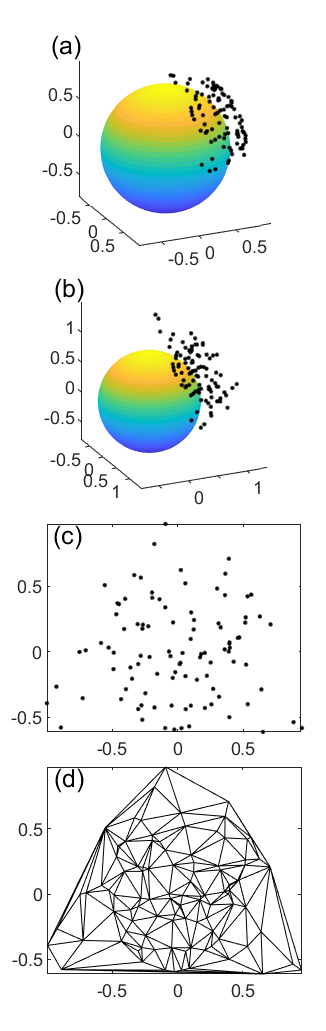
\includegraphics[scale=1]{bary-delaunay.png}
    \caption{3D Cartesian to 2D Cartesian analogue of 7D Cartesian to 6D Cartesian mesh triangulation used in barycentric interpolation approach. Input points linearly projected projected onto hyperplane tangent to mean of starting points (a), degenerate dimension removed via rigid \gls{svd} transformation to 2D Cartesian and Delaunay triangulation calculated (b), and Delaunay triangulation superimposed onto normalized input points. The spheres in (a) and (c) have a radius of 0.8 and is used for visualization only.}
    \label{fig:bary-delaunay}
\end{figure}

% In order to reduce the computationally complexity of computing barycentric coordinates in a high-dimensional space \cite{barberQuickhullAlgorithmConvex1996}, a single degenerate dimension (originally introduced by analytically minimizing $U(1)$ symmetry) is removed to enable use of MATLAB's quickhull \cite{barberQuickhullAlgorithmConvex1996} implementations such as \texttt{delaunayn} and \texttt{convhulln}. Removal of the degenerate dimension is done via a rigid \gls{svd} transformation, analogous to a Cartesian rotation and translation. Thus, a set of octonions originally represented by 8D Cartesian coordinates are collapsed to a 7D Cartesian representation while preserving both distances and angles among the points (see 3D to 2D analogue in \cref{fig:bary-remove-deg}). To further reduce the "curse of dimensionality" in computing the triangulation, a 7D Cartesian representation of the octonions constrained to lie on the surface of the 6-sphere are first projected onto a hyperplane tangent to the mean of the input points and then rotated/translated again via \gls{svd} to produce a 6D Cartesian representation (see 3D to 2D analogue in Figure \cref{fig:bary-delaunay}). This 6D representation is used to compute a triangulation via the built-in MATLAB routine \texttt{delaunayn} based on the quickhull algorithm \cite{barberQuickhullAlgorithmConvex1996}, giving facet vertices for the 7D Cartesian hypersphere.

\subsection{Intersections in a \glsentrytitlecase{vfz}{long} Mesh}
\label{app:bary-int}
An intersection is calculated by linearly projecting a prediction point onto the hyperplane defined by a mesh facet's vertices (\cref{fig:bary-interp}, computing barycentric coordinates within the facet, and testing for positivity \cite{langerSphericalBarycentricCoordinates2006}, and repeating this process until an intersection is found or a stop condition is reached (see \texttt{nnMax} below). If the prediction point is contained within the simplex, all of the barycentric weights (i.e. coordinates) are positive. If it outside the simplex, this constraint is violated. Due to the large number of facets per point of a high-dimensional
%simplex-based
triangulation
%and for computational speed,
prediction point intersections are calculated by considering facets connected to up to some number of mesh \glspl{nn} (\texttt{nnMax}) (in this work, \texttt{nnMax = 10}). For prediction points where no intersecting facet is found
%in these connected facets due to high-aspect ratio facets or prediction point falling outside the mesh within a given tolerance,
a \gls{nn} approach is used (\cref{sec:methods:interp:nn}), which represent average non-intersection rates of \SI{0.1207 \pm 1.02}{\percent} and \SI{0.68 \pm 0.11}{\percent} for input meshes of \num{388} and \num{50000}, respectively, for \num{10000} query points out of \num{10} trials.

\subsection{Interpolation via Barycentric Coordinates}
\label{app:bary-interp}

Once barycentric coordinates are computed for a prediction point within the input mesh, the interpolated value is found by taking the dot product of the barycentric coordinates and the properties of the corresponding vertices of the intersecting facet via
\begin{equation}
\label{eq:bary-interp}
v=\underset{i=1}{\overset{N}{\sum }}\lambda _i v_i
\end{equation}
where $\lambda$, $v$, $v_i$ and $N$, are the barycentric coordinates, interpolated property, property of the $i$th vertex of the intersecting facet, and number of vertices in a given facet ($N = 7$ for the degeneracy-free 6-sphere). A 2-sphere example is provided in \cref{fig:bary-interp}.

\begin{figure}
    \centering
    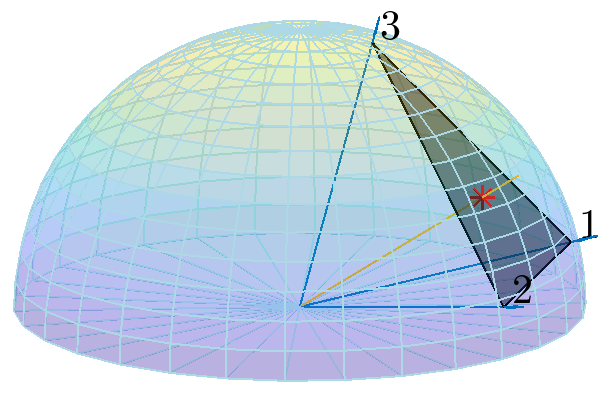
\includegraphics[scale=1]{bary-interp.png}
    \caption{A ray (red line) on the 2-sphere is linearly projected onto the hyperplane of a mesh facet (transparent black), shown as a red asterisk. The barycentric coordinates are computed as $\lambda_{i \in [1,3]} = \frac{1}{3}$. Because all barycentric coordinates are positive, it is determined that the projected point is an intersection with the mesh. Given vertex values of \num{8.183}, \num{3.446}, and \num{3.188} for vertices 1, 2, and 3, respectively, the interpolated value is calculated as \num{4.94} via \cref{eq:bary-interp}.}
    \label{fig:bary-interp}
\end{figure}
	
	% \appendix
	\begin{appendices}
		
		\crefalias{section}{appsec}
		\crefalias{subsection}{appsec}
		\crefalias{subsubsection}{appsec}
		
	\end{appendices}
	
	% \newpage
	\printglossaries
	% \printabbreviations
	%need to manually clear cached files & logs in overleaf to get new abbreviations to appear, maybe?
	
	% \newpage
	\bibliographystyle{elsarticle-num-names}
	\bibliography{5dof-gb-energy.bib}
	
	% \begin{enumerate}
    \item First mesh-based property interpolation scheme that incorporates all five macroscopic crystallographic degrees of freedom.
    \item Past work predicting grain boundary energy
    \begin{enumerate}
        \item \gls{brk} function \cite{Bulatov2014GrainMetals}
        \item Rohrer \gls{gbed} based on binning in nickel \cite{Li2009RelativeNickel}, yttria \cite{Dillon2009CharacterizationFIB}, and copper \cite{Randle2008Five-parameterCopper}. Also \cite{Rohrer2010DerivingData}
        \item other five-parameter articles: titanium \cite{Farabi2018Five-parameterTitanium}, BCC materials \cite{Ratanaphan2015GrainMetals}.
        \item a non-discretizing \gls{knn} approach to determine GB energy \cite{Shen2019DeterminingSpace}.
        \item Neural network predictions \cite{EcheverriRestrepo2014UsingEnergies}
        \item grain boundary octonion theory \cite{Francis2019ABoundaries,Chesser2020LearningProperties}
         \begin{enumerate}
             \item Smooth interpolation between two arbitrary grain boundaries (oSLERP) \cite{Francis2019ABoundaries}
             \item inverse distance weighting approach \cite{Chesser2020LearningProperties}
         \end{enumerate}
    \end{enumerate}
    
    \item extension of octonion representation using barycentric coordinates
    \begin{enumerate}
        \item barycentric coordinates commonly used for interpolation within a simplex or other convex polygon.
        \begin{enumerate}
            \item basic equations (positivity, partition of unity, linear precision) \cite{Langer2006SphericalCoordinates}
        \end{enumerate}
        \item spherical barycentric coordinates that preserve linear precision \cite{Langer2006SphericalCoordinates}, which is important for interpolation, or preserve partition of unity \cite{Lei2020ASystems}, which is better for even subdivision of spherical surfaces.
        \item we incorporate linear precision preserving barycentric coordinates with an octonion representation of GBs to do property interpolation.
    \end{enumerate}
    \item application of this octonion framework using Gaussian process regression
    \begin{enumerate}
        \item Gaussian process regression is a machine learning technique geared towards predicting data (along with prediction intervals and standard deviations of the predictions) for arbitrary regions using a set of input data consisting of predictors and responses.
        \item By supplying a closed octonion mesh, we compute covariance matrices efficiently (i.e. arbitrary distance calculations are very quick), which is important for a Gaussian process regression.
    \end{enumerate}
\end{enumerate}

\section{Results and Discussion} \label{sec:resultsDiscussion}
\begin{enumerate}
    \item parity plots
    \begin{enumerate}
        \item 388 and 50,000 mesh points
        \item tile1 - spherical barycentric interpolation
        \item tile2 - planar barycentric interpolation
        \item tile3 - \gls{gpr}
        \item tile4 - pure \gls{nn} interpolation
    \end{enumerate}
    \begin{figure}
        \centering
        \includegraphics{}
        \caption{parity plots for 388 (red) and 50,000 (black) octonions formed via pairs of random cubochorically sampled quaternion and spherically sampled boundary plane normals. Property values sampled via \acrlong{brk} function and interpolation via barycentric (a), pure \acrlong{nn} (b), and \acrlong{gpr} (c).}
        \label{fig:brk-parity1}
    \end{figure}
    \begin{figure}
        \centering
        \includegraphics{}
        \caption{parity plots for 388 Olmsted \acrfullpl{gb} (red) and 50,000 Kim \acrshortpl{gb} (black) with property values sampled via \acrlong{brk} function and interpolation via barycentric (a), pure \acrlong{nn} (b), and \acrlong{gpr} (c).}
        \label{fig:brk-parity2}
    \end{figure}
    \item \Gls{rmse} vs. number mesh points for barycentric interpolation (black), \gls{gpr}, and pure \gls{nn} interpolation (red). Range from 1e2 to 1e5 mesh points
    \begin{figure}
        \centering
        \includegraphics{}
        \caption{\acrlong{rmse} vs. number of mesh points for spherical barycentric interpolation (black), planar barycentric interpolation, spherical \acrlong{gpr} (red), planar \gls{gpr}, pure \acrlong{nn} interpolation (orange), and average model with standard deviations from 10 random samples.}
        \label{fig:brk-rmse}
    \end{figure}
    \item histograms of \gls{nn} and next \gls{nn} distances (arc length) for mesh
    \begin{figure}
        \centering
        \includegraphics{}
        \caption{histograms of \acrfull{nn} (red) and next \acrlong{nn} (black) arc lengths for meshes of 388 (a), 10,000 (b), and 50,000 (c) octonions formed via pairs of random, cubochorically sampled quaternions.}
        \label{fig:nndist}
    \end{figure}
    \item timing and efficiency
    \begin{enumerate}
        \item fitrgp produces lower error in less time than barycentric interpolation even when using sparse approximation methods.
        \item barycentric interpolation is very fast once the triangulation is computed (i.e. still fast even if responses change, but needs to be recomputed if input data, i.e. predictors, change)
        \item fitrgp is fast and has lower error compared to barycentric interpolation; however, the entire process has to be rerun (in current implementation) if the responses or the predictors change.
    \end{enumerate}
    \item comparison with Chesser \cite{Chesser2020LearningProperties} (few points, Ni data, both high- and low-symmetry sets). Use 388 Ni bicrystals instead of \gls{brk} function. Barycentric and \gls{gpr}
    \begin{enumerate}
        \item table
        \begin{table}[]
            \centering
            \begin{tabular}{c c c c}
                \hline
                 Method & Minimizing Distance & \acrshort{rmse} & \acrshort{mae} \\
                 \hline
                 Barycentric & Euclidean Norm & & \\
                 \acrshort{nn} & Euclidean Norm & & \\
                 \acrshort{gpr} & Euclidean Norm & & \\
                 Pairwise-distance & Arc Length & &
            \end{tabular}
            \caption{Comparison of \acrfull{rmse} and \acrfull{mae} for closed-mesh barycentric interpolation, closed-mesh \acrfull{nn} interpolation, closed-mesh \acrfull{gpr}, and pairwise-distance inverse weighting for 388 Ni bicrystal simulations with 10-fold cross validation for each method.}
            \label{tab:chesser-comp}
        \end{table}
        \item parity plot
        \item \gls{5dof} visualizations
        \begin{figure}
            \centering
            \includegraphics{}
            \caption{\acrfull{gb} energy plotted in the $\Sigma{3}$, $\Sigma{5}$, $\Sigma{7}$, and $\Sigma{11}$ \acrlong{bp} spaces for closed-mesh spherical barycentric (a) and \acrlong{nn} (b) interpolation, closed-mesh \acrlong{gpr} (c), and pairwise-distance inverse weighting using 388 Ni bicrystal simulations.}
            \label{fig:chesser-5dof}
        \end{figure}
        \item 1DOF curves ([100] and [110] symmetric tilt boundaries ?)
    \end{enumerate}
    \item comparison with Restrepo \cite{EcheverriRestrepo2014UsingEnergies} (many points, Fe data, both high- and low-symmetry sets). Use simulated Fe data instead of \gls{brk} function. Barycentric and \gls{gpr}
    \begin{enumerate}
        \item table
        \begin{table}[]
            \centering
            \begin{tabular}{c c c c}
                \hline
                 Method & Minimizing Distance & \acrshort{rmse} & \acrshort{mae} \\
                 \hline
                 Barycentric & Euclidean Norm & & \\
                 \acrshort{nn} & Euclidean Norm & & \\
                 \acrshort{gpr} & Euclidean Norm & & \\
                 \acrshort{ann} & N/A & &
            \end{tabular}
            \caption{Comparison of \acrfull{rmse} and \acrfull{mae} for closed-mesh barycentric interpolation, closed-mesh \acrlong{gpr}, and a non-symmetry considering \acrfull{ann} using 50,000 Fe bicrystal simulations.}
            \label{tab:restrepo-comp}
        \end{table}
        \item parity plot
        \item \gls{5dof} visualizations
        \begin{figure}
            \centering
            \includegraphics{}
            \caption{\acrfull{gb} energy plotted in the $\Sigma{3}$, $\Sigma{5}$, $\Sigma{7}$, and $\Sigma{11}$ \acrlong{bp} spaces for closed-mesh spherical barycentric (a) and \acrlong{nn} (b) interpolation, closed-mesh \acrlong{gpr} (c), and a non-symmetry considering \acrlong{ann} (d) using 50,000 Fe bicrystal simulations.}
            \label{fig:restrepo-5dof}
        \end{figure}
        \item 1DOF curves ([100] and [110] symmetric tilt boundaries ?)
    \end{enumerate}
\end{enumerate}


\section{Methods} \label{sec:methods}

\begin{enumerate}
    \item barycentric interpolation
    \begin{enumerate}
        \item commonly used for interpolation within a simplex or other convex polygon.
        \begin{enumerate}
            \item basic equations (positivity, partition of unity, linear precision) \cite{Langer2006SphericalCoordinates}
        \end{enumerate}
        \item spherical barycentric coordinates that preserve linear precision \cite{Langer2006SphericalCoordinates}, which is important for interpolation, or preserve partition of unity \cite{Lei2020ASystems}, which is better for even subdivision of spherical surfaces.
    \end{enumerate}
    \item Gaussian process regression
    \begin{enumerate}
        \item MATLAB fitrgp
        \begin{enumerate}
            \item squared exponential covariance function
            \item bcd fit method (others are sd, fic etc.)
            \item constant basis function
            \item exact or bcd predict methods (also fic)
            \item quasi-newton optimizer
            \item optimize KernelScale and Sigma hyperparameters with bayesopt Optimizer
            \item ActiveSetMethod - entropy (others, log likelihood, sparse greedy approximation)
        \end{enumerate}
    \end{enumerate}
\item combining octonion representation with barycentric interpolation or Gaussian process regression
    \begin{enumerate}
        \item choosing a symmetrically equivalent representation based on minimum euclidean norm using a single reference octonion (i.e. kept constant)
        \begin{enumerate}
            \item contrast with traditional approach \cite{Francis2019ABoundaries}
            \begin{enumerate}
                \item traditional: allows either octonion to vary for efficiency; ours: one octonion held constant
                \item traditional: use arc length as minimizing metric; ours: use euclidean norm
                \item traditional: consider a subset of symmetrically equivalent GBOs; ours: consider all symmetrically equivalent GBOs
                \item traditional: always stay in 8D representation; ours: remove degenerate dimension (to 7D) for interpolation and employ projections (to 6D) for triangulation efficiency (for barycentric interpolation)
            \end{enumerate}
        \end{enumerate}
        \item triangulating a set of octonions using qhull (for barycentric interpolation)
        \item projections and rotations (projection to hyperplane, singular value decomposition)
        \item spherical barycentric coordinates \cite{Langer2006SphericalCoordinates}
        \begin{enumerate}
            \item equations
        \end{enumerate}
        \item barycentric interpolation
        \begin{enumerate}
            \item equations
            \item Determine intersecting facet using facets connected to \gls{nn}s and positivity constraint of planar barycentric coordinates
            \item intersecting facet vertices projected onto hyperplane tangent to hypersphere at datapoint
            \item containing facet and barycentric coordinates only need to be computed once for each datapoint, can be easily reused
        \end{enumerate}
    \end{enumerate}
    \item random cubochoric sampling \cite{Singh2016OrientationMethods}
    \item use of \gls{brk} function \cite{Bulatov2014GrainMetals}
    
    \item training, validation, and test partitioning \cite{Wang2020MachinePractices} for Kim data set \cite{Kim2011AnDatabase}
    \begin{enumerate}
        \item
    \end{enumerate}
    
\end{enumerate}


\section{Conclusion} \label{sec:conclusion}

\begin{enumerate}
    \item high fidelity interpolation approach is demonstrated
    \item approach is faster than pairwise distance matrices
    \item approach produces lower error than machine learning approach without consideration of symmetrically equivalent GBs
    \item lower error than pure \gls{nn} interpolation
    \item high intersection rate (~99\%) for barycentric interpolation
    \item approach is general to any crystal system and can be controlled by a single parameter (pgnum)
    \item future work
    \begin{enumerate}
        \item extension from linear interpolation to hyperspherical spline interpolation \cite{Taijeron1994SplineHyperspheres}
        \item interpolate within restricted regions of \gls{5dof} space
        \item define true FZ borders (high-symmetry GBs on perimeter)
        \item influence of choice of reference point
        \item influence of regularly spaced points vs. random sampling
        \item extension to generalized spherical barycentric coordinates (i.e. non-simplicial interpolation) \cite{Langer2006SphericalCoordinates}
        \item application to interpolating a GBCD (i.e. like fitting a curve to a histogram) and interpolating other GB properties (e.g. diffusivity, mobility)
        \item use of octonion facet vertices with other distance metrics (i.e. simplex reconstruction using edge lengths \cite{Connor2017High-dimensionalSearch})
        \item distance-based construction of submanifold \cite{Boissonnat2017OnlySubmanifolds}
        \item exploration of other parameters within \gls{gpr}
        \item exploration of machine learning methods other than \gls{gpr}
        \item linking with non-bicrystal data such as Rohrer 3D \gls{tj} data sets (e.g. Ni \cite{Li2009RelativeNickel})
    \end{enumerate}
\end{enumerate}


\section{Supplemental}
\begin{enumerate}
    \item conversion from octonion to \gls{5dof}
    \item high-aspect ratio facets
    \item facet subdivision
    \item spherical vs. planar barycentric interpolation
    \item tolerances of interpolation and intersecting facets
    \item non-intersection percentage vs. number of mesh points
    \item "excess" arc length in pairwise distance matrices
    \begin{enumerate}
        \item gradient optimization and global optimization of U(1) twist symmetry with marginal improvement
    \end{enumerate}
    \item identification and subdivision of hull exterior
    \item distribution of data in \gls{mfz} and \gls{bp} spaces
    \item comments on \gls{gpr} hyperparameters
\end{enumerate}
	
\end{document}
